\documentclass[12pt,letterpaper]{article}

\usepackage[left=1in, right=1in, top=1in, bottom=1in]{geometry}
\usepackage{graphicx}
\graphicspath{{images/}}
\usepackage{mathptmx}
% \usepackage{parskip}
\usepackage{indentfirst}
\usepackage{enumitem}
\usepackage{setspace}
% \usepackage{hyperref}
\usepackage{tabularx}
\usepackage[table]{xcolor}
\usepackage{makecell}
\usepackage{float}
\usepackage{longtable}
\usepackage{subcaption}

\setlength{\parindent}{1.5em}

\begin{document}

\begin{titlepage}

    \centering
    
    \begin{minipage}{6.5in}
        \centering
        \raisebox{-0.5\height}{
\includegraphics[width=0.12\textwidth]{ucf_pegasus_logo.png}}
        \hspace{3em}
        \raisebox{-0.5\height}{
\includegraphics[width=0.75\textwidth]{ucf_bar_logo.png}}
    \end{minipage}
    \vspace{1em}
    
    \textbf{\Large Milestone 3: Concept Design Report}\par\vspace{4em}
    
    \textbf{RDE Senior Design Team 2024-2025}\par\vspace{0.5em}
    Department of Mechanical and Aerospace Engineering\par\vspace{0.5em}
    College of Engineering and Computer Science\par\vspace{3em}
    
    \textbf{Prepared By}\par\vspace{0.5em}
    Paul Dehart, Joshua Kopp, Nathaniel Michnoff, Arturo Negrette, Hunter Quinlan, Egan Rigney, Subhan Wade, Edward Woodruff\par\vspace{3em}
    
    {\bfseries Faculty Advisor}\par\vspace{0.5em}
    Taha Rezzag-Lebza\par\vspace{2em}
    
    
\includegraphics[width=0.4\textwidth]{sabr_logo.png}\par\vspace{2em}
    
    \textit{Due: November 22, 2024}\par\vspace{1em}
    \textit{EAS 4700C / EML 4501C}

\end{titlepage}

\newpage
\thispagestyle{empty}

\section*{Executive Summary}
\doublespacing

Rotating Detonation Engines (RDEs) are a novel method of combusting and accelerating gas for the purpose of rocket propulsion. The function remains similar to conventional rocket engines, as RDEs produce high temperature gas in a combustor that is then expelled through an exhaust wherein the mass flow momentum is used to push the rocket according to Newton’s Laws of Motion. The key difference between RDEs and conventional engines is that the flame front moves beyond the local speed of sound, in a mechanism referred to as “Pressure-Gain Combustion” (PGC). This method of combusting propellants allows for much higher specific impulse, which in turn allows for smaller engines and lower mass-flows to produce equivalent performance when compared to a conventional (constant pressure) engine. The critical aspect of an RDE that allows for this phenomenon to occur is the chamber geometry, ignition, and injector design.


In context of this project, the overarching goal is to design, manufacture, and test fire an architecture capable of using atmospheric air as an oxidizer, and design with features that seek to integrate the system into a flight vehicle. RDEs are far more compact engines that have been shown through extensive research to have major potential as powerplants in hypersonic vehicles, guided munitions, and other compact, high-speed vehicles requiring a high payload to structure mass ratio. The project in its current standing is evaluating the minimum combustor size required to achieve stable detonation based on the propellants selected (Gaseous Hydrogen and Air at 79\% Nitrogen and 21\% Oxygen). Additionally, materials, seals, and injector designs are being selected to maximize efficiency, reduce risk of catastrophic damage to the combustor, and enable reusability of the system.

\singlespacing
\newpage

\tableofcontents

\newpage

\listoffigures

\newpage

\listoftables

\newpage

\section*{Terms and Abbreviations}

\vspace{2em}
\setlength{\tabcolsep}{2.5em}
\begin{center}
    \begin{tabular}{l l}
        CEA & Chemical Equilibrium with Applications \\
        CJ & Chapman-Jouget \\
        CTE & Coefficient of Thermal Expansion \\
        CV & Flow Coefficient \\
        DAQ & Data Acquisition \\
        DDT & Deflagration to Detonation \\
        DFM & Design for Manufacturing \\
        FEA & Finite Element Analysis \\
        FMECA & Failure Modes and Effects Criticality Analysis (A.K.A. FMEA) \\
        FOD & Foreign Object Debris \\
        GH2 & Gaseous Hydrogen \\
        GN2 & Gaseous Nitrogen \\
        GOx & Gaseous Oxygen \\
        GUI & Graphical User Interface \\
        ID & Inner Diameter \\
        IO & Input/Output \\
        JAXA & Japanese Aerospace Exploration Agency \\
        JIC & Jet-in-Crossflow \\
        NASA & National Aeronautics and Space Administration \\
        NI & National Instruments \\
        NPT & National Pipe Thread \\
        OD & Outer Diameter \\
        ORB & O-Ring Boss \\
        OS & Operating System \\
        PERL & Propulsion and Energy Research Lab \\
        PGC & Pressure Gain Combustion \\
        PPE & Personal Protective Equipment \\
        PRV & Pressure Relief Valve \\
        PT & Pressure Transducer \\
        RDE & Rotating Detonation Engine \\
        RTD & Resistance Temperature Detector \\
        RTV & Room-Temperature Vulcanizing \\
        R\&D & Research and Development \\
        SABR & Small-Scale Air-Breathing RDE \\
        SS & Stainless Steel \\
        TC & Thermocouple \\
        UCF & University of Central Florida \\
        U.S.A & United States of America \\
        USB & Universal Serial Bus \\
        ZND & Zeldovich Von Newmann D\"{o}hring \\
    \end{tabular}
\end{center}

\newpage

\section{Introduction}
\doublespacing

Rotating Detonation Engines were initially researched and developed in the 1950s and 60s with the infancy of large-scale rocket propulsion, but due to the lack of understanding of supersonic combustion and lack of high-speed imaging necessary to analyze and study a detonation wave, were mostly left untouched until the turn of the century. Organizations such as JAXA have developed full scale flight prototypes that have shown their potential in orbit, like other more conventional methods of rocket propulsion. However, there is a significant lack of development for RDE use in the atmosphere.

Similarly to ramjets and scramjets, RDEs show promise in use for atmospheric vehicles that can benefit from a lightweight propulsion system that can remain efficient at hypersonic speeds. The motivation behind this project is to develop a system capable of operating in the atmosphere using hydrogen and air. The major problem that comes from running an RDE on atmospheric air composition as the oxidizer comes from the large amount of inert nitrogen being included in the reaction that acts as a heatsink and impedes the detonation to an extent. This project will be addressing this issue by experimenting and iterating through different nitrogen dilution percentages, starting from pure oxygen and arriving at effectively the same conditions seen in the atmosphere.

This report will be focused on the starting parameters of the project, such as the requirements and needs to meet through the development of a combustor, test stand, and feed system capable of achieving the overall goals. Additionally, the existing technologies and the options available for certain components will be explored, leading to the preliminary analysis and modeling needed to set the parameters that will lead the rest of the design in the coming months, which will be outlined with a Gantt chart and further discussion in this report. As with any engineering design, the possible failure modes present with the approach taken will be discussed, and their criticality to the project will be analyzed. Finally, the future work necessary to further refine the design and overall project performance will be studied and possible recommendations for the rest of this track will be explored.

\newpage

\doublespacing
\renewcommand{\arraystretch}{1.25}
\renewcommand{\tabularxcolumn}[1]{m{#1}}
% \newcolumntype{Y}{>{\centering\arraybackslash}}

% ----- SECTION 2: NEEDS ANALYSIS -----
\newpage
\section{Needs Analysis}
\subsection{Propulsion \& Energy Research Laboratory}

The primary end user of our system will be the researchers at the Propulsion \& Energy Research Laboratory (PERL). The results, findings, and lessons learned of Project SABR will be directly used for further development of this capability. The hardware paid for by the department will remain at PERL for future use, as well.

The goals for this project are to design, build, and test a small-scale air-breathing RDE and its facility, achieve detonation during testing with Hydrogen as the fuel, record load cell data from the test, build an operational map for the combustor, and not sustain significant damage after use. These achievements will be incredibly useful in the characterization of the combustor and will provide insight into the design of the next version and its testing. 

\subsection{Research and Development Programs}

The potential stakeholders of Project SABR are the RDE research and development programs across the country. The ability to study the complicated phenomena associated with RDE operation in air-breathing mode at a fraction of the typical cost will inevitably increase the R\&D activity in this type of propulsion and power generation. The demonstration of a small-scale air-breathing RDE using Hydrogen as fuel will also increase greater interest in realizing this technology.

% TODO: Add reference to section 5 in this paragraph
The stakeholders’ interests in Project SABR include the demonstration of a small-scale RDE using Hydrogen and air, design and demonstration of a unique ignition method for RDEs, the formulation of an operational map of the combustor, and recommendations for future work and designs. After conversations with industry professionals, showing that detonation is possible with air in a small-scale combustor would be incredibly useful to the community. The second most useful outcome of the project would be the novel use of an ignition method in an RDE that would allow for an optimized form factor. This is explored more in Section 5: [Igniter Concept Generation]. The last two products mentioned of the project provide the community with insight into the next problems that need to be tackled for the realization of this technology.

\subsection{Potential Customers}

The potential customers of this system are the U.S. government, NASA, government contractors and other private companies in the aerospace and power generation industries. The inclusion of RDEs in governmental materials and commercial products would decrease the amount of hardware, volume, and weight required for a given work output. Thus, the system itself would cost less, have better performance, and simplify the engineering process (given the current problems at hand are solved). 

The main challenges to overcome with making this a viable product is the reliability of the combustor, the form factor of the supporting systems, the storage of hydrogen fuel, and the cooling of the combustion chamber. There are ongoing and rapidly developing efforts for cooling methods and hydrogen storage methods for operational systems. The reliability of the combustor will be observed during our testing campaign. Our project also aims to explore solutions to the form factor problem with the ignition method.

% ----- SECTION 3: NEEDS ANALYSIS -----
\newpage
\section{Technology Assessment}
\subsection{Injector}

The overarching purpose of an injector is to introduce the propellants into the combustor and mix them as homogeneously as possible. There is not much variation between injectors for RDEs and conventional engines from a fundamental standpoint, as all compressible gas dynamics relations still apply when it comes to orifice sizing and performance. However, certain nuances apply that allow for easier initiation of the detonation wave. Similar to conventional deflagration-based engines, the most basic type of injector geometry is impinging. Impinging injectors feature two streams of propellant colliding into a singular spray cloud, allowing for atomization of liquid propellants, as well as mixing for both gaseous and liquids. The mixing is determined by the angles and relative mass flows of each element. Mixing efficiency is directly connected to relative velocities between the propellants, as the overall goal is to introduce shear between the two with the intent of generating turbulence.

Jet-in-Crossflow injection consists of one of the propellants being injected axially, while the other one is injected radially so the jets meet at 90 degrees from one another. This induces a large amount of mixing for a relatively simple geometry and allows for the propellant chosen to go through the center body possibly being used for regenerative cooling. JIC also allows for partial pre-mixing, where the jets are allowed to meet in a small cavity before transitioning to the annulus.

Mixing efficiency has been experimentally proven to correlate with detonation aspects such as wave speed, wave propagation, as well as conventional parameters such as thrust and specific impulse. Bigler et al. \cite{bigler:2019} demonstrates the effects tied to these parameters, with one of the highlights being that improper mixing leads to counter-rotating waves, which are unfavorable due to their association with lower operating frequencies and wave speeds. These effects are also heavily dependent on local equivalence ratios. A combustor environment with poorly mixed propellants has experimentally been shown to have much more of an impact on wave propagation than the overall equivalence ratio \cite{bigler:2019}. Another alternative injection method is a pre-mixed jet. This method involves mixing the two propellants in a pre-injection chamber or plenum. By mixing upstream of injection, the gases are in contact with each other for a longer period (residence time). The mixing chamber also allows the two gases to reach near stagnation properties while occupying the same space, which results in higher gas-gas diffusion rates and allows for a near uniform mixture before the propellants even enter the chamber. The drawback of this is creating a potentially explosive mixture in the plenum with a high risk of explosion due to the partial backflow characteristic of RDEs.

\vspace{1em}
\noindent The critical aspects for a successful and efficient injector design come down to the following:

\begin{enumerate}[label=(\alph*)]
    \item Well-mixed propellants yield the best benefits in terms of thrust and specific impulse, similar to conventional engines.
    \item Smaller orifices with higher diodicity contribute to better injector replenishment rates, and reduced backflow in the environment directly downstream of the detonation wave.
    \item Choked injectors tend to isolate the detonation waves from the feed system and help increase detonation stability
    \item Efficient injectors yield fewer but stronger detonation waves.
    \item Injector design remains critical to achieve long term detonation stability and needs to be carefully chosen to meet the overarching goals for the RDE. Additionally, a proactive approach towards design for manufacturing and refurbishment capabilities is beneficial to maximize the testing time and the ability to recover from damage and erosion to internal engine components.
\end{enumerate}
\subsection{RDE Combustor}

RDEs are a developing form of propulsion and power generation that utilize the radial propagation of detonation waves within an annulus to combust propellants. These combustors have been proven to work with a combination of solid, liquid, and gas fuels with liquid or gas oxidizers. They can run in either an air-breathing or rocket modes. Additionally, small-scale rocket RDE combustors have been demonstrated as feasible; however, much work remains to characterize their operation with different sizes, propellant combinations, and operating conditions due to the remaining work that needs to be conducted on detonation physics and how it changes in RDEs with high curvature.

Detonation is one of two forms of combustion (deflagration and detonation) that uses reacting, propagating shockwaves to combust reactants. The detonation thermodynamic cycle, the Zeldovich-von Neumann-Döring (ZND) cycle, shows a pressure gain during the heat addition process, which provides a greater work output. This principle is why RDEs are such an attractive technology. If a higher work output per propellant mass is achieved, it can decrease the cost and weight required for a system as well as its environmental impact.

The ZND detonation model is characterized by a compression wave followed by a reaction zone, then an expansion wave. When the compression wave interacts with reactants, there exists a spike in pressure, density, and temperature of the chemical species. This in turn induces high pressure combustion and volume expansion, which causes the compression wave to propagate. The wave then propagates at a theoretical velocity, called the Chapman-Jouguet (CJ) velocity. This velocity can be determined by applying the definition of the Mach number (Ma) to the upper CJ point, which is the intersection of the Rankine and Hugoniot lines.

In practice, the velocity experienced in RDEs is about 60\% of the CJ velocity.  The explanation as to why this occurs is still heavily debated, but it is theorized that it is attributed to parasitic deflagration, where reactants combust due to deflagration. Due to the detonation combustion not being present in all the propellant injected, there is not an ideal pressure rise. This causes a decrease in the pressure applied to the compression wave. Thus, it does not propagate at the ideal theoretical speed.

In aircraft engines, the performance parameters are typically the thrust generated, the specific impulse, the work output, and the thermodynamic efficiency. For a combustor, the means of optimizing these are through the achieving full combustion by optimizing parameters such as equivalence ratio, mass flow rate, and the dimensions of the combustor. However, there are some additional unique parameters that affect RDEs.

It has been shown that detonation cell size is correlated to the overall performance of RDEs. This is because if the detonation cell size is large compared to the annular gap, there will not be enough detonation cells to induce new cell formation and thus wave propagation. This cell size is highly dependent on the propellant mixture and the pressure of the mixture prior to wave interaction.

Various propellants have been tested in RDEs, especially small-scale RDEs. For the case of Project SABR, we will be using air as an oxidizer. Thus, the fuel chosen must optimize the key performance parameters of RDEs. The limiting parameter for our operation is the detonation cell size. The two fuels that have cell sizes small enough for a small-scale RDE are Hydrogen and Methane. From experimental data, it is shown that the cell size of Hydrogen is an order of magnitude smaller than Methane at our desired operating pressure, and thus will maximize our ability to achieve an ideal operation. Additionally, Hydrogen requires less energy input than Methane to induce detonation, and thus is a desirable choice.

Small-scale RDEs have been tested with a variety of designs and propellants. There are a series of theses from the Air Force Institute of Technology that have built on designs and reported challenges faced during operation. Additionally, they provide a template for small-scale RDE design for combustion, stabilization, injection, and material choice. Thus, their findings will play a heavy role in contextualizing our design approach.

Additionally, a three-inch RDE using air and Hydrogen was tested for operating condition limits in a collaboration between researchers in Beijing, China and Warsaw, Poland. It found stable detonation, quasi-stable detonation, unstable detonation, and fast-deflagration combustion for a variety of mass flow rates and pressure ratios. They also studied the detonation wave dynamics during their operation. Their findings for optimal operation will serve as guardrails in our desired flow properties.

Overall, detonation combustion is a very useful and efficient process of providing work to a system. The combination of physical, chemical, and thermodynamic models will lead to the definition of key performance parameters. This analysis can be complicated, but by using and customizing proven methods, it can be done relatively easily. Applying the known detonation properties of fuels to key performance parameter definitions and related equations, the resultant values should be compared to inform the decision on which fuel to use. Additionally, the phase at which the propellants are injected into the combustor may have an impact on performance, and thus should be taken into consideration during the analysis and/or decision-making process. Using proven methods of analysis, reviewing past successes and failures, and the effect of performance parameters on other design choices will assist in improving the quality of the system and the engineering process.
\subsection{Testing Characteristics}

The purpose of this technology assessment is to provide background information on test characteristics and their impact on the project. This document will introduce the characteristics requiring testing, outline the fundamental principles of testing flight profiles, discuss relevant laws, standards, and physics behind simulating an air breathing engine. Additionally, it will examine the impact these factors have on the ready-to-integrate RDE project thus far. The contents of the following information is the guide that has been utilized in the requirements definition process, the design and information of our system architecture, and has facilitated further investigations into the testing of the RDE and related topics.

In the development of the SABR project thus far, we have remained cognizant of the ready-to-integrate standard for our engineering prototype of an RDE. We have further developed the proper testing characteristics that are essential to understand and simulate, as data acquisition and processing will allow us to develop an operational map of the complex and extreme operating conditions these engines face. RDEs function on the principle of continuous supersonic detonation waves, making them more efficient compared to traditional rocket engines. However, their unique combustion process introduces significant challenges, such as high thermal loads, pressure fluctuations, and detonation stability, all of which must be carefully assessed through testing.

Throughout much of the project cycle thus far, we have focused our attention on the flight profile and simulation capabilities of our system. We have based our design around a gas oxidizer fed system that will be diluted with nitrogen to achieve an air mixture ratio. To properly assess our experiment, we are comparing the inlet conditions with the dynamically changing atmosphere. Our rocket engine has been designed to withstand the constantly changing variables of the properties of the gas fed oxidizer. The flight profile presented plays a role with this selection of operation, as we want to be able to test operative capability at potentially different compositions of the atmosphere. Additionally, our exit geometry has been modified through the flight profile assessment. We sought to utilize a nozzle that is capable of operation at variable altitudes and therefore variable static pressures. As aircraft ascend in altitude, air density decreases and changes the pressure that the exhaust gases experience. This can greatly impact the efficiency of these engines; therefore, a consideration of nozzle types was determined to be necessary. Properly accounting for these changing factors is critical for optimizing the engine performance across various flight stages.
\subsection{Data Acquisition and Control}

Data acquisition is the backbone of any experimental setup. The accuracy and reliability of the collected data determine the extent to which conclusions can be drawn from the experiments conducted. Strategic placement of thermocouples, pressure transducers, mass flow meters, flow controllers, load cells, and other instruments is required to evaluate and document critical test parameters and outcomes.  These sensors are read and translated using a DAQ device, each of which has a maximum sampling rate and a maximum number of channels that sensors can occupy. These parameters will determine how the DAQ is configured and what sensors can be utilized in this system.

Several factors play a critical role in this project and although all the topics presented in the technology study memo are important, one of the most vital of these is the sampling rate. This is because the rest of the parameters heavily rely on high-quality top-of-the-shelf sensors which is not a luxury we can afford. Sampling rate, on the other hand, can be easily changed and is set by the DAQ itself. The specific DAQ model we purchased (NI USB-6210) has the capability to do up to 250 kS/s. However, this is not 250 kS/s per channel, this is the total combined sampling rate across all channels. Due to the quick operation time and short duration of our tests, a high sampling frequency is recommended to observe the full scope of phenomena that are occurring within the system. In reality, sampling at a rate of 10 kS/s per channel would be more than sufficient for our sensors.

Another consideration when designing the data acquisition schematic is the number of DAQ channels. This is also a highly important topic as it determines how many total sensors we can utilize in our system. With the selected hardware (NI USB-6210) we have a total of 16 analog voltage inputs (±10 V), four (4) digital inputs, and four (4) digital outputs. The analog input channels are where the sensors will reside and thus are the most important here. The analog channels can be run in either a single-ended or differential configuration. Single-ended only utilizes one channel per sensor, using the common ground as the reference. While this allows the use of all 16 channels, it introduces a significant amount of noise in the resultant data. Differential, on the other hand, uses the common from the sensor as the reference voltage, thus producing a much cleaner signal but occupies two channels per sensor. After assessing the needs of each sub-system, we have decided to proceed with the differential configuration for all sensors. The total number of sensors we need at this stage is minimal and can be reduced to fit within the 8-channel maximum, five (5) pressure transducers for the feed lines and plenum to determine inlet mass flow rates, and three (3) load cells to measure the thrust output of the system.

With these DAQ restrictions in mind, the sensor selection may begin. However, given the budget constraints there will likely only be a few options. However, the following sensor parameters still greatly affect how the data acquisition is implemented and understood. Accuracy, resolution, range, sampling rate, and response time all play a critical role in sensor selection. Accuracy is defined as the maximum difference that will exist between the actual value and the indicated value at the output of the sensor \cite{ni-fundamentals:2023}. Sensors often provide users with an accuracy specification in which they are accurate within a range of values. However, in addition to this confidence interval, calibration, scaling, and signal shielding must be taken into account to produce accurate measurements.

The resolution of a sensor is the smallest detectable incremental change of input parameter that can be detected in the output signal \cite{ni-fundamentals:2023}. The resolution of a sensor is critical, if the incorrect sensor is selected, it may not pick up on small changes in the system and miss key findings. The range of a sensor determines its measuring limits. If a given sensor is exposed to conditions outside its measurement range, it will likely permanently damage the sensor. Thus, when selecting a sensor, analysis should be conducted in order to derive theoretical minimums and maximums that each sensor will see.

Similar to the resolution, sampling rate is highly important as it determines the level of granularity that can be seen in a system. A slow sampling rate may be adequate for monitoring some systems, but for systems with rapid variations like a RDE, a slow sampling rate would not capture the micro-second changes that are occurring in the system. Response time is defined by the time it takes a sensor to respond to a change in the system state. This reaction time, if too long, can cause the measurement system to completely miss quick phenomenon that are occurring.

Data acquisition is the most important thing when it comes to experimental testing. Without clear, concise, and reliable data the results of an experiment are left unsupported. To procure reliable data, the optimal selection of sensors must be completed by quantifying expected outputs and selecting sensors that adhere to the accuracy, resolution, range, sampling rate, and response time requirements of the system. These sensor selection parameters can be applied to the small-scale RDE system to evaluate critical measurements such as fuel flow rate, oxidizer flow rate, specific impulse, fuel injection parameters, and wave propagation speed.
\subsection{Test Stand Configuration}

The purpose of this technology assessment is to provide background information on the design requirements for a test stand tailored to small-scale air-breathing rotating detonation engines and their impact on the project as a whole. This document will outline the essential principles of test stand design and assembly, describe relevant technologies for thrust measurement, and explore their implications for the successful testing of RDEs. The following information has guided the process of further defining our project requirements, informed system architecture development, and enabled further investigations into the testing and evaluation of test stand technology.

Over the course of the project thus far, the focus has been on designing a test stand capable of meeting the structural, measurement, and operational demands that are unique to RDEs. Unlike conventional rocket engines, RDEs generate thrust though supersonic detonation waves, which introduces many more unique challenges to the process of designing and developing an adequate test stand for this use. These factors require a specialized approach to test stand design, enabling reliable structural stability and high accuracy thrust data collection over the course of multiple tests. As we continue to work towards a functional hot fire test of a small-scale RDE, we have focused our attention down to two primary areas when it comes to test stand development: the stand must provide stability to minimize the effects of external forces on the engine’s performance and must be able to measure the thrust produced by the engine to a high level of accuracy. By addressing these core areas, the test stand will be able to serve as a reliable platform for characterizing the performance and operational behavior of the RDE.

One of the most obvious and important features for the test stand to exhibit is the ability to combine robustness with adaptability, being able to support the engine under extreme operating conditions. Throughout much continued research, two frequently used techniques for structurally supporting the engine emerged, serving as great methods for this task while remaining within the manufacturing and budgetary limits constraining the project. One such method is to mount the engine on a set of linear rails, which would in turn constrain the engine’s motion to a single linear axis, better directing thrust forces into load cells for accurate measurement. This idea has remained very popular in test stand design due to its ability to nearly eliminate all external lateral forces, which would otherwise distort thrust measurements. Another popular design is to mount the engine to a “floating” plate that is only connected to the rest of the test stand’s static structure via the load cells. This solution achieves the same effect of eliminating external lateral forces almost as well as the rail-based design but comes with the added benefit of being much cheaper and easier to fabricate.

Another extremely important feature that the test stand must include is a system to calibrate load cells, something that must be done prior to testing to ensure that the thrust data being collected is accurate. There were two popular methods for this that emerged as well, both with similar benefits and limitations, making the choice between the two options rely on external project limitations. One method is to utilize a hydraulic ram and associated static structure which can attach to the load transfer structure, or even the RDE itself, and apply a known force to test and calibrate the load cells. A similar result can be obtained with the much simpler, but less efficient, mass and pulley calibration system in which weights of known mass can be attached to a cord running over a pulley and attaching to the back of the load transfer structure in order to calibrate the load cells. With these multiple options, it is absolutely crucial to ensure that the load cells are able to accurately measure the exact thrust being produced by the RDE.

While the specific configurations of the test stand may not entirely control the development of the RDE system on its own, the choices made to achieve the two important test stand functions do have a large impact on the rest of the project, mainly though budgetary, manufacturing, and timeline restrictions. For each configuration option for the test stand, there is a balance between data accuracy and cost/complexity, and in many cases due to the timeline and budget of the project, the slightly cheaper and less complex option may be chosen, as long as it can be ensured that the main project requirements are still being met. In addition, the different options have a large impact on the adaptability of the test stand, as some configurations may be able to better accommodate future modifications to the RDE at the cost of more expensive and complicated designs.

In conclusion, while the test stand is not critical to the function of the RDE itself, it is extremely crucial to the successful development, evaluation, and implementation of RDE technology. By continuing to narrow and address the most important functions of the test stand, the ability to thoroughly test the engine and its unique operational characteristics will provide plenty of data to inform the design, optimization, and validation of RDE systems. Drawing from these existing designs will allow the test stand to support the rigorous demands of RDE testing and contribute to the overall success of this project.
\subsection{Fluid Systems}

There are many considerations when it comes to the design of the feed system for a small-scale air-breathing rotating detonation engine. The goals of project SABR are to design, build and test the RDE and determine the ranges of total mass flow rate and equivalence ratios over which the RDE can operate and produce stable detonation. This section will introduce and cover propellant feed systems in the context of the project as well as the fundamental principles of fluidic hardware, fluid flow, and the safety and handling of high-pressure systems.

Small size RDEs reduce the requirements for fuel and oxidizer flow rates, which makes the RDE more portable and easier to iterate upon \cite{dechert:2020}. This is due to the fact that small-scale RDEs have small channel geometries, which inherently results in lower mass flow rates and higher frequencies of operation \cite{dechert:2020, fiorino:2021, fiorino:2022}. One of the biggest challenges will be refreshing propellants at a high enough rate into the chamber with enough time and energy for proper reactant mixing. This will mainly fall under the responsibility of the injector. However, it will help to have a precise, steady, and repeatable feed of propellants into the injector plenums to help reduce transience in the system. Flow rates are acquired through relations between detonation cell size, chamber radii, channel widths, combustor lengths, and operational frequencies. Equivalence ratios are a result of chemical equilibrium considerations and will be calculated to maximize the reaction efficiency. \cite{yokoo:2019}. Given an equivalence ratio and associated propellant mass flow rates, as well as desired plenum pressures the feed system becomes simplified, focusing solely on providing and recording the mass flow rates and pressures with high accuracy and consistency.

\begin{figure}[ht]
    \centering
    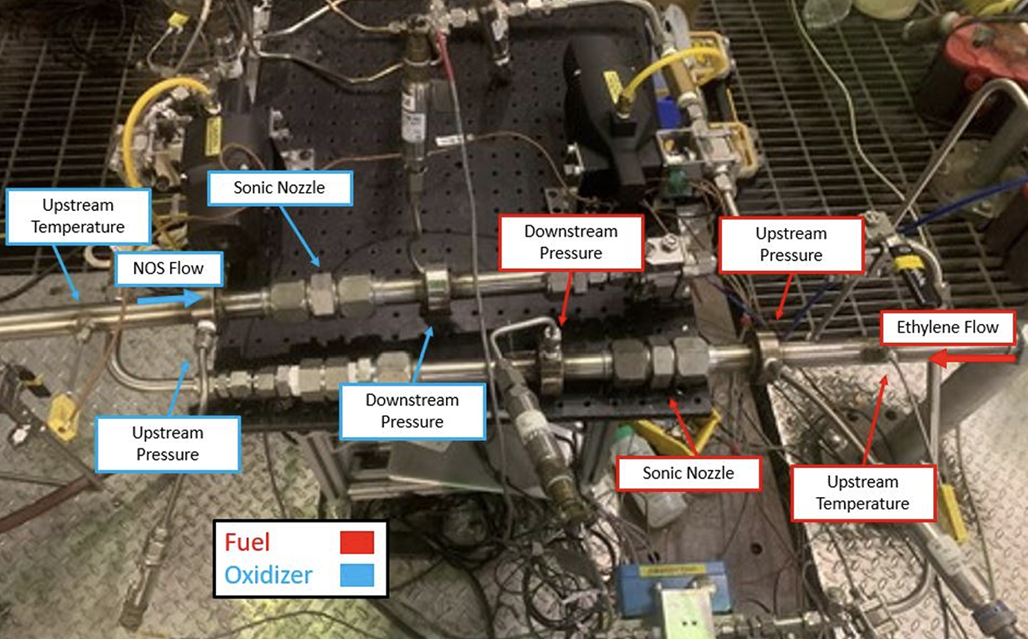
\includegraphics[width=0.75\linewidth]{rde_feed_system_example.png}
    \caption{Example of an RDE feed system (from Wyatt)}
    \label{fig:rde-feed-system-example}
\end{figure}

As mentioned before, one of the primary difficulties with feed systems for small scale RDEs is that the reactants must be supplied into the detonation channel at a rate fast enough so that they are refreshed prior to each passing wave \cite{dechert:2020, fiorino:2021, fiorino:2022}. The amount of time available to refresh the reactants can be extremely short in RDEs. It is even shorter when you consider that the detonation wave passing over the injector inlets can temporarily block the flow of fuel and oxidizer through the injector into the detonation channel due to its extreme pressures \cite{dechert:2020}. The total mass flow rate that of propellants that needs to be provided to the engine will come from the engine specifications. Required mass flow rates of propellants for the detonation reaction has dependence on cell size, fill height, channel length, and channel gap \cite{dechert:2020, fiorino:2021, connolly-boutin:2021, bykovskii:2012}. To determine the detonation frequency for a given RDE, the detonation velocity must be known. Detonation velocity can be a function of many factors to include fuel/oxidizer type and equivalence ratio \cite{dechert:2020, bykovskii:2012}. The detonation cell size is important since the necessary height of the fresh propellants for sustained detonation is directly related to the cell size \cite{bykovskii:2012, russo:2011}.

Changes in mass flow rates have been found to have significant effects on the detonation reaction, especially on the number of waves \cite{law:2021}. At low mass flows create fewer wave detonation at lower frequencies \cite{fiorino:2022, law:2021}. Equivalence ratio and mass flow rates will be calculated using isentropic flow equations and mass flow rate equations such as shown in Figure 2 \cite{nasa-mass-flow-choking:2021, nasa-mass-flow-equations:2021}. Conditions will be calculated upstream using reservoir conditions and readings from pressure gauges. Flow restrictions such as regulators and orifices will be used to control flow rates.

In prior testing with RDEs it has been shown that mass flow instruments have a difficult time accurately measuring mass flow rates due to the pressure oscillations and transient conditions of the flow. It has been shown that sonic orifices can be used to successfully measure mass flow rates by choking the flow at the orifice. Using upstream conditions and the dimensions of the orifice, a mass flow rate can be calculated. When this flow rate is time averaged over the length of the test, it has been shown to produce accurate measurements.

To simulate air-breathing conditions, three feed lines will be used. O$_2$ and GN$_2$ lines will be mixed upstream of the injector to simulate different oxidizer dilutions, with the ultimate goal being a 79\% dilution of the oxygen to simulate air as the oxidizer. All three lines will be similar in setup, using sonic orifices to control and measure mass flow rates. There will also be other lines extending off of the propellant lines which will be used to feed the pre-detonation/ignition system. Plenums allow for the fuel and oxidizer to be distributed to the injector holes of the injector plate. Plenum to chamber pressure ratios determine chocked flow conditions at the injector and can influence the characteristics of the detonation \cite{fiorino:2022, yokoo:2019}. Flow will be sonic at the injector holes because the pressure difference will be controlled to be large enough to meet sonic conditions.

Choking is typically assumed at the injectors. However, the propagation of the detonation wave creates regions of high pressure downstream which could temporarily disturb the choking conditions causing pressures in the line to increase to sustain mass flow rates into the chamber \cite{yokoo:2019}. Otherwise, if the injector is choked, plenum pressures should remain constant. As the detonation wave passes over the injector holes, the high pressure can force products back into the fuel/oxidizer plenum which would have adverse effects on the equivalence ratio and the stability of the detonation wave \cite{dechert:2020}. Therefore, it is critical that choking conditions are achieved at the injector inlet and that the pressures in the plenum allow for this.

The flow of oxidizer and fuel will require flow control devices and a precise control system. Valves of different types will be considered and implemented to reach these requirements. To have precise and repeatable control, solenoid valves will be controlled with DAQ hardware and a driving software to send valve actuation signals. The test setup will also record flow, pressure, temperature, and thrust data.

Understanding the effects of friction on fluid flow through the piping system will be crucial for optimal performance. Parameters such as the coefficient of discharge area (C$_d$A) or flow coefficient (C$_v$) will be used to characterize pressure drops across flow restrictions such as bends in tubing, valves, and orifices \cite{crane-co:1982, asme-fluid-flow:2004, nasa-tubing:2019}. Bends and fittings in the tubing, rough inner surfaces, and restrictions from valves will contribute to energy losses in the system. It will be essential to design and model the flow paths to ensure proper pressures and mass flow rates throughout the system.

Several different types of fluidic connections will likely be used in the system. These could include compression, such as Swagelok, ORB (O-ring boss), NPT (National Pipe Thread), cone-and-thread, and flared fittings (such as JIC 37-degree). Due to the high-pressure applications in this system, Swagelok and NPT fittings are the most likely to be used, as they have some of the best sealing abilities under extreme conditions. The system will incorporate stainless steel tubing of varying thickness to accommodate the different pressure ranges and flow rates that will be required. These parameters will need to be balanced carefully to minimize pressure drops across the system, ensure proper seals, and optimize the safety and performance of the engine.

During the testing phase, the team will be handling high-pressure fluids, including oxidizers like oxygen (O$_2$), fuels such as hydrogen (H$_2$) and inert gases such as gaseous nitrogen (GN$_2$). Given the hazardous nature of these fluids, strict precautions will be implemented during storage and interactions. Oxygen, as an oxidizer, increases the risk of combustion in the presence of flammable materials, necessitating specialized handling procedures and oxygen-safe environments. Inert gases like GN$_2$, while non-flammable, will still be managed under high-pressure conditions, requiring careful attention to equipment and safety protocols to prevent leaks or failures. All personnel will follow rigorous safety guidelines, including personal protective equipment (PPE) use, continuous monitoring of pressure levels, and adherence to standardized handling procedures for high-pressure gases \cite{aiga-hydrogen-supply:2024, aiga-oxygen-cleaning:2019, nasa-oxygen-systems:1996}.

This project will involve managing extremely high temperatures and pressures, especially when dealing with the detonation reaction. The system will also have potentially hazardous combustion products, including gases containing fine particulate matter. The team must utilize proper pressure fittings that are compatible with these fluids and rated for these conditions to minimize the risk of leaks, failures, and contamination from foreign object debris (FOD). The presence of small solid particles and other material poses a significant risk for contaminating the system, especially considering the very small areas at which flows will be choked or reach sonic conditions. These contaminants can cause pressure buildups, reduce flow rates, and damage components, all of which could cause catastrophic failure of the system. To mitigate these risks, the team will implement proper cleaning procedures, particularly oxygen cleaning, to ensure oxidizer-safe environments and prevent clogging or build-up of material in the flow paths \cite{aiga-oxygen-cleaning:2019}. Maintaining clean lines will be essential for both the team’s safety and the engine's health.

Managing high pressures is a fundamental aspect of this system's design. Over-pressurization presents a severe risk to both the system and personnel. Therefore, pressure relief valves (PRVs) and burst discs will be incorporated into the fluid system to provide a fail-safe for excessive pressure buildup. PRVs will open automatically to release pressure when it exceeds safe limits and burst discs will rupture at a specific pressure threshold, providing an emergency pressure release mechanism. The feed system will be designed to have pressure relief lines to prevent trapped pressure, and valves will be selected to ensure that they fail into “safe” positions in the event of power losses. Pressure relieving components and careful system design are critical for ensuring the safety of the system and of operators during hazardous operations. 

In conclusion, designing the feed system for a small-scale air-breathing rotating detonation engine involves several significant challenges. The engine’s reliance on pressure gain combustion means precise control of mass flow rates, equivalence ratios, and reactant mixing is critical. These challenges are amplified in small-scale systems, where limited space and rapid refresh rates make achieving stable detonation more difficult. Careful consideration of fluid dynamics, appropriate hardware, and safety measures will be essential to ensure the engine operates efficiently and safely in these extreme conditions.

The success of this project depends on developing a robust feed system that can handle high pressures and temperatures while preventing the backflow of detonation products. Selecting the right fittings, flow control valves, and pressure management tools will be crucial for maintaining safe and stable operation. Additionally, special attention to factors such as friction, contaminants, and pressure drops will help ensure consistent fuel and oxidizer flow, optimizing engine performance. This approach will provide the necessary groundwork for designing, building, and testing an RDE capable of stable detonation under a variety of conditions, advancing the understanding and development of pressure gain combustion technologies.
\subsection{Igniter}

Deflagrations and detonations are both mechanisms of combustion by which a mixture of fuel and an oxidizer release heat into a system. The fundamental difference being that deflagrations are associated with flame fronts propagating at subsonic velocities (in the context of rocket engines, the flame front is equal to the injection velocity which is usually on the order of 10-100 meters per second) while detonations propagate at supersonic velocities, often on the order of several to tens of kilometers per second, depending on the mixture chemistry and density. Because detonations propagate at supersonic speeds, a shock wave forms in front of the combustion zone which compresses and raises the temperature of the fuel-oxidizer mixture in front which then detonates and continues the reaction. It should be noted that the wave speed and pressure rise associated with detonations is proportional to the density of the reactants. For reference, gas/gas reactants can yield pressure rises in the several or tens of thousands of psi, while liquid/liquid reactants can easily achieve detonation pressure on the order of millions of psi and significantly higher detonation velocities \cite{heister:2022}.

The transition from deflagration to detonation and the following propagation of detonation waves depends on several factors, but almost always driven by how properly mixed the reactants are in a control volume. If we imagine a long tube filled with an air-fuel mixture that is then ignited by some external means, the resulting flame will initially travel at subsonic speeds through the tube. As the deflagration propagates, it begins to accelerate due to minor gains in velocity from shock reflection, shock focusing, or instabilities/interaction between the flame front and mach waves \cite{breitung:2000} (an infinitely weak shock wave, if enough mach waves stack upon each other due to compressible effects, it creates a shock wave). If the deflagration accelerates long enough it will eventually evolve into a full detonation wave. However, this process requires a tube of considerable L/D ratio so the characteristic length must be long enough for the deflagration to accelerate.

Pre-detonation igniters are devices that take advantage of DDT phenomena to ignite RDEs. They work by filling a long tube with reactants (usually the same mixture being fed into the main chamber, just tapped off the main lines) and ignited via spark ignition. The mixture will then undergo DDT, generating a detonation wave by the time the flame front leaves the tube and enters the combustor. Because pre-detonation igniters generate a shock, only a single firing is required to startup an RDE. However, they do require a separate feed and valve system which poses some challenges for integration and packaging constraints.

Deflagration to detonation phenomenon gives us several avenues towards the development of a reliable ignition method for our proposed engine. A pre-detonation ignition system works by filling a tube connected to the combustor with reactants, which is then ignited via spark igniter. The reactants eventually undergo a transition from deflagration to detonation given enough tube length where the resulting detonation wave is fed into the combustor. This provides the engine with a strong initial detonation wave and has been experimentally observed to be a more reliable method of engine startup. A direct-spark ignition system is more compact than a pre-detonation system as it does away with the relatively long length of tube required to initiate a deflagration to detonation transition. A direct-spark ignition system involves directly threading the spark plug into the combustor, using the detonation channels as the characteristic length needed to promote a detonation transition. While it is a much simpler method, a recessed spark plug has been experimentally shown to be unreliable, often failing to transition the deflagration flame front to a detonation. On the other hand, a spark plug whose electrode is extruding into the chamber suffers from erosion due to constant exposure to the detonation waves \cite{dechert:2020} and requires replacement after only several firings. These characteristic strengths and weaknesses must be considered in the design process of our engine, as a poor ignition method can hamper the progress during our test campaign and restrict the cadence of firings.

% ----- SECTION 4: SYSTEM REQUIREMENTS -----
\newpage
\section{System Requirements}
\renewcommand{\tabcolsep}{6pt}
\singlespacing

\subsection{SABR Requirements}

% ----- SABR REQUIREMENTS -----
\begin{table}[H]
    \centering
    \small
    \begin{tabularx}{\linewidth}{
        |>{\hsize=0.100\linewidth}>{\centering\arraybackslash}X
        |>{\hsize=0.150\linewidth}>{\centering\arraybackslash}X
        |>{\hsize=0.400\linewidth}>{\centering\arraybackslash}X
        |>{\hsize=0.175\linewidth}>{\centering\arraybackslash}X
        |>{\hsize=0.175\linewidth}>{\centering\arraybackslash}X|
    }
        \hline
        \textbf{ID} & \textbf{NAME} & \textbf{Description} & \textbf{Requirement Type} & \textbf{Verification Method} \\ \hline

        SABR-1 & Thrust & SABR shall produce measurable thrust. & Functional & Test \\ \hline
        
        SABR-2 & Detonation & SABR shall demonstrate capability of detonation. & Functional & Test \\ \hline

        SABR-3 & Oxidizer & SABR should operate using atmospheric air composition (79\% N$_2$, 21\% O$_2$). & Functional & Test \\ \hline

        SABR-4 & System Scale & SABR shall scale its components and perform metrics to a small scale compared to current operational systems. & Performance & Analysis \\ \hline

        SABR-5 & Reusability & SABR should not sustain extensive damage for the duration of engine burn. & Sustainability & Demonstration \\ \hline

        SABR-6 & System Interface & SABR shall interface with the equipment provided by PERL. & Interface & Inspection \\ \hline

        SABR-7 & Operational Verification & SABR shall be static fire tested at a regime of propellant and dilutant conditions to build an operational map of the RDE. & Verification & Demonstration \\ \hline

        SABR-8 & System Cost & SABR should not exceed a cost of \$1,000. & Cost & Inspection \\ \hline

    \end{tabularx}
    \caption{SABR Requirements}
    \label{tab:sabr_requirements}
\end{table}

\subsection{RDE Requirements}

% ----- RDE FUNCTIONAL REQUIREMENTS -----
\begin{table}[H]
    \centering
    \small
    \caption{RDE System Requirements}
    \label{tab:rde_requirements}

    \begin{subtable}[t]{\linewidth}
        \begin{tabularx}{\linewidth}{
            |>{\hsize=0.175\linewidth}>{\centering\arraybackslash}X
            |>{\hsize=0.200\linewidth}>{\centering\arraybackslash}X
            |>{\hsize=0.450\linewidth}>{\centering\arraybackslash}X
            |>{\hsize=0.175\linewidth}>{\centering\arraybackslash}X|
        }
            \hline
            \textbf{ID} & \textbf{Name} & \textbf{Description} & \textbf{Verification Method} \\ \hline
        
            SABR-RDE-1 & Ignition & SABR-RDE shall employ a means for detonation ignition. & Inspection \\ \hline
        
            SABR-RDE-2 & Injection & SABR-RDE shall inject propellants at a specified mass flow rate. & Analysis \\ \hline
        
            SABR-RDE-3 & Flow Stabilization & SABR-RDE shall stabilize flow conditions received from SABR-TS. & Analysis \\ \hline
        
            SABR-RDE-4 & Thrust Structure & SABR-RDE shall withstand thrust generated. & Demonstration \\ \hline
        
            SABR-RDE-5 & Active Cooling	& SABR-RDE may use regenerative cooling to extend operation time. & Analysis \\ \hline

        \end{tabularx}
        \smallskip
        \caption{RDE System Functional Requirements}
    \end{subtable}
\end{table}

\vspace{-1em}

% ----- RDE PERFORMANCE REQUIREMENTS -----
\begin{table}[H]
    \centering
    \small
    \ContinuedFloat

    \begin{subtable}[t]{\linewidth}
        \begin{tabularx}{\linewidth}{
            |>{\hsize=0.175\linewidth}>{\centering\arraybackslash}X
            |>{\hsize=0.200\linewidth}>{\centering\arraybackslash}X
            |>{\hsize=0.450\linewidth}>{\centering\arraybackslash}X
            |>{\hsize=0.175\linewidth}>{\centering\arraybackslash}X|
        }
            \hline
            \textbf{ID} & \textbf{Name} & \textbf{Description} & \textbf{Verification Method} \\ \hline
        
            SABR-RDE-6 & Startup Time & SABR-RDE should transition the combustion mode to detonation within ten (10) milliseconds of ignition. & Test \\ \hline

            SABR-RDE-7 & Material Selection & SABR-RDE shall be manufactured out of materials that withstand operating conditions. & Analysis \\ \hline

            SABR-RDE-8 & Mass Flow & SABR-RDE should inject propellants at a combined mass flow of at least 50 g/s. & Analysis \\ \hline

            SABR-RDE-9 & Thrust & SABR-RDE should produce measurable thrust in the range of 75 – 250 N. & Test \\ \hline

            SABR-RDE-10 & Propellants & SABR-RDE should perform reliably while approaching atmospheric air as an oxidizer (79\% N$_2$ - 21\% O$_2$). & Test \\ \hline
            
            SABR-RDE-11 & Operational Time & SABR-RDE should run in detonation mode for at least 0.25 seconds. & Test \\ \hline

        \end{tabularx}
        \smallskip
        \caption{RDE System Performance Requirements}
    \end{subtable}
\end{table}

\vspace{-1em}

% ----- RDE INTERFACE REQUIREMENTS -----
\begin{table}[H]
    \centering
    \small
    \ContinuedFloat

    \begin{subtable}[t]{\linewidth}
        \begin{tabularx}{\linewidth}{
            |>{\hsize=0.175\linewidth}>{\centering\arraybackslash}X
            |>{\hsize=0.200\linewidth}>{\centering\arraybackslash}X
            |>{\hsize=0.450\linewidth}>{\centering\arraybackslash}X
            |>{\hsize=0.175\linewidth}>{\centering\arraybackslash}X|
        }
            \hline
            \textbf{ID} & \textbf{Name} & \textbf{Description} & \textbf{Verification Method} \\ \hline
        
            SABR-RDE-12 & Propellant Interface & SABR-RDE shall receive propellants delivered from SABR-TS. & Demonstration \\ \hline
    
            SABR-RDE-13 & Structural Interface & SABR-RDE shall transfer thrust to the test stand's structure. & Analysis \\ \hline
            
            SABR-RDE-14 & Data Acquisition Interface & SABR-RDE shall include necessary sensor ports for integration with data acquisition. & Demonstration \\ \hline

        \end{tabularx}
        \smallskip
        \caption{RDE System Interface Requirements}
    \end{subtable}
\end{table}

\vspace{-1em}

% ----- RDE VERIFICATION REQUIREMENTS -----
\begin{table}[H]
    \centering
    \small
    \ContinuedFloat

    \begin{subtable}[t]{\linewidth}
        \begin{tabularx}{\linewidth}{
            |>{\hsize=0.175\linewidth}>{\centering\arraybackslash}X
            |>{\hsize=0.200\linewidth}>{\centering\arraybackslash}X
            |>{\hsize=0.450\linewidth}>{\centering\arraybackslash}X
            |>{\hsize=0.175\linewidth}>{\centering\arraybackslash}X|
        }
            \hline
            \textbf{ID} & \textbf{Name} & \textbf{Description} & \textbf{Verification Method} \\ \hline
        
            SABR-RDE-15 & Interface Verification & SABR-RDE shall undergo interface verification of its components and subassemblies. & Inspection \\ \hline

            SABR-RDE-16 & Functional Verification & SABR-RDE shall undergo functional verification of its components and subassemblies. & Demonstration \\ \hline
            
            SABR-RDE-17 & Performance Verification & SABR-RDE shall undergo performance verification of its components and subassemblies. & Test \\ \hline
            
            SABR-RDE-18 & Manufacturability Verification & SABR-RDE shall undergo manufacturability verification of its components and subassemblies. & Analysis/Test \\ \hline

        \end{tabularx}
        \smallskip
        \caption{RDE System Verification Requirements}
    \end{subtable}
\end{table}

\vspace{-1em}

% ----- RDE OTHER REQUIREMENTS -----
\begin{table}[H]
    \centering
    \small
    \ContinuedFloat

    \begin{subtable}[t]{\linewidth}
        \begin{tabularx}{\linewidth}{
            |>{\hsize=0.175\linewidth}>{\centering\arraybackslash}X
            |>{\hsize=0.200\linewidth}>{\centering\arraybackslash}X
            |>{\hsize=0.450\linewidth}>{\centering\arraybackslash}X
            |>{\hsize=0.175\linewidth}>{\centering\arraybackslash}X|
        }
            \hline
            \textbf{ID} & \textbf{Name} & \textbf{Description} & \textbf{Verification Method} \\ \hline
        
            SABR-RDE-19 & Operational Safety & SABR-RDE shall not introduce significant risk to the test operators or the testing environment. & Inspection \\ \hline
    
            SABR-RDE-20 & Manufacturability & SABR-RDE shall be designed to maximize the manufacturing capabilities available to the team. & Demonstration \\ \hline
            
            SABR-RDE-21 & Sustainability & SABR-RDE shall be sustainable in a manner that is convenient to service and build upon. & Analysis \\ \hline

        \end{tabularx}
        \smallskip
        \caption{RDE System Other Requirements}
    \end{subtable}
\end{table}

\subsection{Test Stand Requirements}

% ----- TEST STAND FUNCTIONAL REQUIREMENTS -----
\begin{table}[H]
    \centering
    \small
    \caption{Test Stand System Requirements}
    \label{tab:ts_requirements}

    \begin{subtable}[t]{\linewidth}
        \begin{tabularx}{\linewidth}{
            |>{\hsize=0.175\linewidth}>{\centering\arraybackslash}X
            |>{\hsize=0.200\linewidth}>{\centering\arraybackslash}X
            |>{\hsize=0.450\linewidth}>{\centering\arraybackslash}X
            |>{\hsize=0.175\linewidth}>{\centering\arraybackslash}X|
        }
            \hline
            \textbf{ID} & \textbf{Name} & \textbf{Description} & \textbf{Verification Method} \\ \hline
        
            SABR-TS-1 & Imaging Diagnostics & SABR-TS should collect imaging diagnostics at a point downstream of the exhaust to validate the presence of detonations & Demonstration \\ \hline
    
            SABR-TS-2 & Pressure Diagnostics & SABR-TS shall collect pressure diagnostics at various points throughout the system & Demonstration \\ \hline
            
            SABR-TS-3 & Temperature Diagnostics & SABR-TS shall collect temperature diagnostics at various points throughout the system & Demonstration \\ \hline
            
            SABR-TS-4 & Load Cell Diagnostics & SABR-TS should measure applied loads with an accuracy of ±3\% & Demonstration \\ \hline
            
            SABR-TS-5 & Structural limits & SABR-TS shall withstand all applied force and vibrational forces in a static loading case. & Analysis \\ \hline
            
            SABR-TS-6 & Sustainability & SABR-TS shall be sustainable in a manner that is convenient to service and build upon. & Analysis \\ \hline
            
            SABR-TS-7 & Engine Support & SABR-TS-STR shall provide mounting and support for the engine. & Demonstration \\ \hline
            
            SABR-TS-8 & Fluid System Support & SABR-TS-STR shall provide mounting and support for the fluid system. & Demonstration \\ \hline
            
            SABR-TS-9 & Electronics Support & SABR-TS-STR shall provide mounting and support for the electronics. & Demonstration \\ \hline
            
            SABR-TS-10 & Transportable & SABR-TS-STR shall be transportable. & Demonstration \\ \hline
            
            SABR-TS-11 & Loads & SABR-TS-STR shall be able to withstand all loads. & Demonstration \\ \hline
            
            SABR-TS-12 & Loads on Fluid System & SABR-TS-STR shall be able to reduce structural loads on the Fluid System. & Analysis \\ \hline

        \end{tabularx}
        \smallskip
        \caption{Test Stand System Functional Requirements}
    \end{subtable}
\end{table}

\vspace{-1em}

% ----- TEST STAND PERFORMANCE REQUIREMENTS -----
\begin{table}[H]
    \centering
    \small
    \ContinuedFloat

    \begin{subtable}[t]{\linewidth}
        \begin{tabularx}{\linewidth}{
            |>{\hsize=0.175\linewidth}>{\centering\arraybackslash}X
            |>{\hsize=0.200\linewidth}>{\centering\arraybackslash}X
            |>{\hsize=0.450\linewidth}>{\centering\arraybackslash}X
            |>{\hsize=0.175\linewidth}>{\centering\arraybackslash}X|
        }
            \hline
            \textbf{ID} & \textbf{Name} & \textbf{Description} & \textbf{Verification Method} \\ \hline
        
            SABR-TS-13 & Thrust measurements & SABR-TS thrust plate assembly shall be able to measure applied loads up to 5 kN with a resolution of 0.5 N. & Analysis \\ \hline
    
            SABR-TS-14 & Form Factor & SABR-TS components should fit within a standard-size SUV trunk volume. & Inspection \\ \hline

            SABR-TS-15 & Manufacturability & SABR-TS structural components shall consist of widely available metal extrusions. & Inspection \\ \hline

            SABR-TS-16 & Weight & SABR-TS-STR shall be able to support a weight of 250 N. & Analysis \\ \hline
            
            SABR-TS-17 & Thrust Loads & SABR-TS-STR shall maintain a minimum factor of safety of five (5) at all times. & Analysis \\ \hline

        \end{tabularx}
        \smallskip
        \caption{Test Stand System Performance Requirements}
    \end{subtable}
\end{table}

\vspace{-1em}

% ----- TEST STAND INTERFACE REQUIREMENTS -----
\begin{table}[H]
    \centering
    \small
    \ContinuedFloat

    \begin{subtable}[t]{\linewidth}
        \begin{tabularx}{\linewidth}{
            |>{\hsize=0.175\linewidth}>{\centering\arraybackslash}X
            |>{\hsize=0.200\linewidth}>{\centering\arraybackslash}X
            |>{\hsize=0.450\linewidth}>{\centering\arraybackslash}X
            |>{\hsize=0.175\linewidth}>{\centering\arraybackslash}X|
        }
            \hline
            \textbf{ID} & \textbf{Name} & \textbf{Description} & \textbf{Verification Method} \\ \hline
        
            SABR-TS-18 & Combustor Interface & SABR-TS shall physically interface with the combustor via the thrust plate. & Inspection \\ \hline

            SABR-TS-19 & Feed System Interface & SABR-TS shall supply structural support and relevant physical interfaces to feed system outlets. & Inspection \\ \hline

            SABR-TS-20 & DAQ Interface & SABR-TS shall provide the necessary electrical power and data transmission capabilities to all sensors within the system domain. & Inspection \\ \hline

            SABR-TS-21 & Lab Interface & SABR-TS shall be physically secured within the allocated lab space at PERL. & Inspection \\ \hline

        \end{tabularx}
        \smallskip
        \caption{Test Stand System Interface Requirements}
    \end{subtable}
\end{table}

\vspace{-1em}

% ----- TEST STAND OTHER REQUIREMENTS -----
\begin{table}[H]
    \centering
    \small
    \ContinuedFloat

    \begin{subtable}[t]{\linewidth}
        \begin{tabularx}{\linewidth}{
            |>{\hsize=0.175\linewidth}>{\centering\arraybackslash}X
            |>{\hsize=0.200\linewidth}>{\centering\arraybackslash}X
            |>{\hsize=0.450\linewidth}>{\centering\arraybackslash}X
            |>{\hsize=0.175\linewidth}>{\centering\arraybackslash}X|
        }
            \hline
            \textbf{ID} & \textbf{Name} & \textbf{Description} & \textbf{Verification Method} \\ \hline
        
            SABR-TS-22 & Control System Complexity  & SABR-TS control system shall be easily operable and free from unnecessary complexities  & Demonstration \\ \hline

        \end{tabularx}
        \smallskip
        \caption{Test Stand System Other Requirements}
    \end{subtable}
\end{table}

\subsection{Fluid System}

% ----- FLUID SYSTEM FUNCTIONAL REQUIREMENTS -----
\begin{table}[H]
    \centering
    \small
    \caption{Fluid System Requirements}
    \label{tab:fs_requirements}

    \begin{subtable}[t]{\linewidth}
        \begin{tabularx}{\linewidth}{
            |>{\hsize=0.175\linewidth}>{\centering\arraybackslash}X
            |>{\hsize=0.200\linewidth}>{\centering\arraybackslash}X
            |>{\hsize=0.450\linewidth}>{\centering\arraybackslash}X
            |>{\hsize=0.175\linewidth}>{\centering\arraybackslash}X|
        }
            \hline
            \textbf{ID} & \textbf{Name} & \textbf{Description} & \textbf{Verification Method} \\ \hline
        
            SABR-FS-1 & Propellant Flow Rate Control & SABR-FS shall control flow rates for each propellant. & Test \\ \hline
    
            SABR-FS-2 & Oxidizer Composition Modulation & SABR-FS shall fine tune and vary the oxidizer mixture. & Test \\ \hline
            
            SABR-FS-3 & System Purging & SABR-FS shall be capable of purging all lines with an inert gas. & Demonstration \\ \hline
            
            SABR-FS-4 & SABR-RDE Propellant Supply & SABR-FS shall supply SABR-RDE with propellants. & Demonstration \\ \hline

            SABR-FS-5 & SABR-TS Propellant Supply & SABR-FS shall supply SABR-TS with propellants. & Demonstration \\ \hline

        \end{tabularx}
        \smallskip
        \caption{Fluid System Functional Requirements}
    \end{subtable}
\end{table}

\vspace{-1em}

% ----- FLUID SYSTEM PERFORMANCE REQUIREMENTS -----
\begin{table}[H]
    \centering
    \small
    \ContinuedFloat

    \begin{subtable}[t]{\linewidth}
        \begin{tabularx}{\linewidth}{
            |>{\hsize=0.175\linewidth}>{\centering\arraybackslash}X
            |>{\hsize=0.200\linewidth}>{\centering\arraybackslash}X
            |>{\hsize=0.450\linewidth}>{\centering\arraybackslash}X
            |>{\hsize=0.175\linewidth}>{\centering\arraybackslash}X|
        }
            \hline
            \textbf{ID} & \textbf{Name} & \textbf{Description} & \textbf{Verification Method} \\ \hline
        
            SABR-FS-6 & Oxidizer Supply & SABR-FS shall deliver oxidizer mass flow to combustor between 50-200 g/s. & Analysis \\ \hline

            SABR-FS-7 & Fuel Supply & SABR-FS shall deliver fuel mass flow to combustor between 1-10 g/s. & Analysis \\ \hline

            SABR-FS-8 & Structural Stability & SABR-FS shall be able to withstand nominal operating conditions. & Demonstration \\ \hline

            SABR-FS-9 & SABR-RDE Propellant Mixture & SABR-FS shall provide SABR-RDE with a mixture of propellants in the equivalence ratio range of 0.8 to 1.2 and in the Nitrogen dilution range of 0\% to 79\%. & Test \\ \hline

            SABR-FS-10 & SABR-TS Propellant Mixture	& SABR-FS shall provide SABR-RDE with a mixture of propellants in the equivalence ratio range of 0.8 to 1.2 and in the Nitrogen dilution range of 0\% to 79\%. & Test \\ \hline

        \end{tabularx}
        \smallskip
        \caption{Fluid System Performance Requirements}
    \end{subtable}
\end{table}

\vspace{-1em}

% ----- FLUID SYSTEM INTERFACE REQUIREMENTS -----
\begin{table}[H]
    \centering
    \small
    \ContinuedFloat

    \begin{subtable}[t]{\linewidth}
        \begin{tabularx}{\linewidth}{
            |>{\hsize=0.175\linewidth}>{\centering\arraybackslash}X
            |>{\hsize=0.200\linewidth}>{\centering\arraybackslash}X
            |>{\hsize=0.450\linewidth}>{\centering\arraybackslash}X
            |>{\hsize=0.175\linewidth}>{\centering\arraybackslash}X|
        }
            \hline
            \textbf{ID} & \textbf{Name} & \textbf{Description} & \textbf{Verification Method} \\ \hline
        
            SABR-FS-11 & SABR-RDE Interface & SABR-FS shall integrate with SABR-RDE. & Inspection \\ \hline

            SABR-FS-12 & SABR-TS Interface & SABR-FS shall integrate with SABR-TS. & Inspection \\ \hline

            SABR-FS-13 & PERL Interface & SABR-FS shall integrate with the PERL systems. & Inspection \\ \hline

        \end{tabularx}
        \smallskip
        \caption{Fluid System Interface Requirements}
    \end{subtable}
\end{table}

\vspace{-1em}

% ----- FLUID SYSTEM VERIFICATION REQUIREMENTS -----
\begin{table}[H]
    \centering
    \small
    \ContinuedFloat

    \begin{subtable}[t]{\linewidth}
        \begin{tabularx}{\linewidth}{
            |>{\hsize=0.175\linewidth}>{\centering\arraybackslash}X
            |>{\hsize=0.200\linewidth}>{\centering\arraybackslash}X
            |>{\hsize=0.450\linewidth}>{\centering\arraybackslash}X
            |>{\hsize=0.175\linewidth}>{\centering\arraybackslash}X|
        }
            \hline
            \textbf{ID} & \textbf{Name} & \textbf{Description} & \textbf{Verification Method} \\ \hline
        
            SABR-FS-14 & Cold Flow Verification & SABR-FS shall be cold flow tested at the nominal flow conditions. & Demonstration \\ \hline
    
            SABR-FS-15 & Integration Verification & SABR-FS shall undergo integration verification of its components and sub assemblies. & Inspection \\ \hline

        \end{tabularx}
        \smallskip
        \caption{Fluid System Verification Requirements}
    \end{subtable}
\end{table}

\vspace{-1em}

% ----- FLUID SYSTEM OTHER REQUIREMENTS -----
\begin{table}[H]
    \centering
    \small
    \ContinuedFloat

    \begin{subtable}[t]{\linewidth}
        \begin{tabularx}{\linewidth}{
            |>{\hsize=0.175\linewidth}>{\centering\arraybackslash}X
            |>{\hsize=0.200\linewidth}>{\centering\arraybackslash}X
            |>{\hsize=0.450\linewidth}>{\centering\arraybackslash}X
            |>{\hsize=0.175\linewidth}>{\centering\arraybackslash}X|
        }
            \hline
            \textbf{ID} & \textbf{Name} & \textbf{Description} & \textbf{Verification Method} \\ \hline
        
            SABR-FS-16 & Safing Procedure & SABR-FS shall shutdown or fail in a safe condition. & Demonstration \\ \hline

        \end{tabularx}
        \smallskip
        \caption{Fluid System Other Requirements}
    \end{subtable}
\end{table}

\doublespacing

% ----- SECTION 5: CONCEPT GENERATION AND SELECTION -----
\newpage
\section{Concept Generation and Selection}

\subsection{RDE Trade Studies}
\subsubsection{Combustor Material Study}

The chamber of an RDE contains the inner body, the outer body, the annulus gap, and any interfaces with diagnostic instrumentation, injectors, plenums, and the nozzle/aerospike. The material selection for this assembly is very important as the hot gases flowing through the annulus will reach temperatures and pressures around 3000K and 1600psi (11 MPa). With increased temperature, the yielding strength of materials greatly decreases. Additionally, materials tend to oxidate much more rapidly when exposed to high temperature combustion. 

A trade study was conducted to determine the ideal chamber material for the SABR system dependent upon the cost, schedule, risk, manufacturability, and technical performance. It considered Copper and 304 Stainless Steel, as recommended by industry professionals. The relevant requirements were derived and reported to assist in contextualizing this trade study, Next, evaluation criteria were decided based on the factors that affect the success of the system, project functions, and safety of operators. Then, the evaluation scales and weights were determined based on their expected effects on the same factors used to define the evaluation criteria. Measures of Performance were defined to induce a scientific approach to the technical performance scoring. Finally, each option was evaluated and input into a decision matrix, where an optimal material was defined.

\noindent\underline{Option 1: Copper 110}

\noindent\textit{Pros:}

Copper is often used for combustion chambers due to its heat sink capabilities. This is a function of its thermal conductivity. During operation, copper’s high thermal conductivity (about 400 W/m-K) allows heat to be transferred at a high rate from the inner surface to the outer surface. Thus, active cooling methods can be maximized. Additionally, cooling after operation can be maximized with a high thermal conductivity due to a higher heat transfer rate than materials with a lower thermal conductivity. 

The common availability of copper also contributes to its favorability. If any roadblocks introduce themselves during procurement, it is important to pivot to alternative vendors. Copper stock can be delivered within one week of purchase.

Due to copper’s low rating on the hardness scales, expensive tooling is not required; however, it can be damaged due to its high ductility. This opens the opportunity for mistakes during manufacturing, integration, and testing processes. These risks are much less impactful than a material that ranks high on the hardness scale, though.

\noindent\textit{Cons:}

Copper’s high price compared to other commonly available metals may make its acquisition infeasible. The group currently possesses a quote for one foot of 4-inch-diameter copper stock for about \$550. Under the assumption that the group would receive \$1,000 in funding, the procurement of this material would severely impact the budget available for the other systems and components.

Also, copper’s yield strength at high temperatures is potentially a cause for concern. The yield strength of pure copper at room temperature is about 70 MPa, but it decreases greatly with temperature as seen in Figure \ref{fig:metallic-materials-strength}. Given that the nominal conditions are expected to be about 11 MPa, other material options should be considered. It is still a viable option as prior work has demonstrated that this effect is negligible for short duration tests; however, more research must be done to be sure of its passing of yield strength under nominal conditions.

\begin{figure}
    \centering
    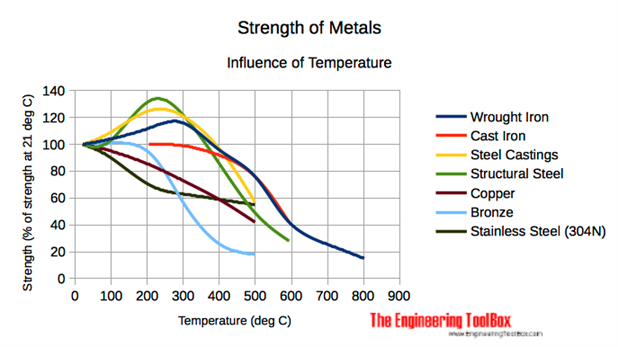
\includegraphics[width=0.8\linewidth]{metallic_materials_strength.png}
    \caption{Strength of metallic materials as a function of temperature.}
    \label{fig:metallic-materials-strength}
\end{figure}

The melting point of copper is about 1400 K. The expected nominal conditions are at about 3000 K. Thus, alternative material options should be considered. Prior work has shown that this is negligible for short duration tests, though. This concern may be mitigated with the use of regenerative cooling, but the inclusion of such design introduces additional complexity to the systems and integration.

The technical performance of copper in the application of our system can be characterized by its thermal conductivity, yield strength at nominal temperature, melting point, and indentation hardness on the Rockwell B scale. It performs very well in thermal conductivity, but it lacks the ability to withstand operational pressures and temperatures on its own. The use of this material for the combustor will lean on the external sources of cooling as is common in liquid rocket engines. This capability has been proven in adjacent engine configurations, and there is current work in the industry to realize this cooling method for RDEs.

\noindent\underline{Option 2: 304 Stainless Steel}

\noindent\textit{Pros:}

Stainless steel is attractive as a material option mainly due to its low cost. For a 4-inch diameter and 14 in. in length stock of 304 Stainless Steel, it costs about \$200. The procurement of this material would allow more expensive purchases in other systems. Also, if more stock needs to be ordered, the price will not be too detrimental to the outcome of the project.

304 Stainless Steel has a yield strength of 215 MPa. It also has a nominal yield strength of 75 MPa at 1170K. This is much higher than the operating pressure of 11 MPa, and thus is a viable option for medium duration run time (greater than 1 second but less than 10 seconds). This capability would be helpful in testing the time effects on operational capability.

Additionally, 304 Stainless Steel has a melting point of about 1725K. This would potentially contribute to higher operational times without the need for complex cooling systems. It can also help increase the amount of test cases for short duration runs.

\noindent\textit{Cons:}

304 Stainless Steel is not great for cooling, though. It has a thermal conductivity of 21.5 W/m-K. Thus, regenerative cooling would be fairly infeasible with non-cryogenic fluids. However, cooling may not be necessary for our operational setting with the high melting point and high yield stress of this material.

Another drawback of 304 Stainless Steel is the challenges with machining. It has a high work hardening rate, which requires machining procedures to be much more precise. However, this high strength means that ductility effects during machining won’t be as much of a concern.

Finally, 304 Stainless Steel tends to oxidate at high temperatures when working with pure oxygen. However, when using higher Nitrogen percentages, this concern becomes negligible. This limits our operational conditions to a range of nitrogen dilution close to and including that of air.

The technical performance of 304 Stainless Steel in the application of our system can be characterized by its thermal conductivity, yield strength at nominal temperature, melting point, and indentation hardness on the Rockwell B scale. It performs fairly well in all categories except for thermal conductivity. The use of this material for the combustor will lean on the ability to withstand pressures and temperatures rather than external sources of cooling. This capability has been proven in heritage systems and will leverage their design approaches.

% ----- CRITERIA & WEIGHTS -----
\begin{table}[H]
    \centering
    \singlespacing
    \small
    \caption{Combustor Material Trade Study - Evaluation Criteria}
    \label{tab:combustor_material_eval_criteria}

    \begin{subtable}[t]{\linewidth}
        \begin{tabularx}{\linewidth}{
            |>{\hsize=0.200\hsize}>{\centering\arraybackslash}X
            |>{\hsize=0.100\hsize}>{\centering\arraybackslash}X
            |>{\hsize=0.700\hsize}>{\centering\arraybackslash}X|
        }
            \hline
            \textbf{Decision Criteria} & \textbf{Weight} & \textbf{Reason} \\ \hline

            Cost & 30\% & The combustion chamber is one of many components included in SABR. Thus, the cost of this assembly must be as low as possible while meeting proper performance standards. \\ \hline
        
            Schedule & 10\% & The lead time necessary for stock must be as low as possible to start machining the components as soon as possible. This will allow proper time for integration and V\&V events. \\ \hline
        
            Risk & 15\% & This component should not introduce significant risk for the operation of SABR. \\ \hline

            Manufacturability & 15\% & The ease of manufacturing will allow a shorter lead time on machining and mitigate accidents during those processes \\ \hline
        
            Technical Performance & 25\% & The material chosen for the combustion chamber must withstand operational conditions. \\ \hline
        \end{tabularx}
        \smallskip
        \caption{Evaluation Criteria and Weights}
    \end{subtable}

\end{table}

\vspace{-2em}

% ----- COST SCALE -----
\begin{table}[H]
    \centering
    \singlespacing
    \small
    \ContinuedFloat

    \begin{subtable}[t]{0.5\linewidth}
        \begin{tabularx}{\linewidth}{
            |>{\hsize=0.250\hsize}>{\centering\arraybackslash}X
            |>{\hsize=0.750\hsize}>{\centering\arraybackslash}X|
        }
            \hline
            \textbf{Score} & \textbf{Reason} \\ \hline
            
            5 & \$0 - \$100 \\ \hline
            4 & \$100 - \$200 \\ \hline
            3 & \$200 - \$300 \\ \hline
            2 & \$300 - \$400 \\ \hline
            1 & \$400 and above \\ \hline
        \end{tabularx}
        \smallskip
        \caption{Evaluation Scale - Cost}
    \end{subtable}
\end{table}

\vspace{-2em}

% ----- SCHEDULE SCALE -----
\begin{table}[H]
    \centering
    \singlespacing
    \small
    \ContinuedFloat

    \begin{subtable}[t]{0.5\linewidth}
        \begin{tabularx}{\linewidth}{
            |>{\hsize=0.250\hsize}>{\centering\arraybackslash}X
            |>{\hsize=0.750\hsize}>{\centering\arraybackslash}X|
        }
            \hline
            \textbf{Score} & \textbf{Reason} \\ \hline
            
            5 & 0 - 1 week \\ \hline
            4 & 1 - 2 weeks \\ \hline
            3 & 2 - 3 weeks \\ \hline
            2 & 3 - 4 weeks \\ \hline
            1 & 4 weeks and longer \\ \hline
        \end{tabularx}
        \smallskip
        \caption{Evaluation Scale - Schedule}
    \end{subtable}
\end{table}

\vspace{-2em}

% ----- RISK SCALE -----
\begin{table}[H]
    \centering
    \singlespacing
    \small
    \ContinuedFloat

    \begin{subtable}[t]{0.8\linewidth}
        \begin{tabularx}{\linewidth}{
            |>{\hsize=0.150\hsize}>{\centering\arraybackslash}X
            |>{\hsize=0.850\hsize}>{\centering\arraybackslash}X|
        }
            \hline
            \textbf{Score} & \textbf{Reason} \\ \hline
        
            5 & Does not pose any threat \\ \hline
            4 & Does not pose any threat if mitigated measures are in place \\ \hline
            3 & Poses some threat if mitigated measures are in place \\ \hline
            2 & Poses significant threat when mitigations are in place \\ \hline
            1 & Threats are not able to be mitigated \\ \hline

        \end{tabularx}
        \smallskip
        \caption{Evaluation Scale - Risk}
    \end{subtable}
\end{table}

\vspace{-2em}

% ----- MANUFACTURABILITY SCALE -----
\begin{table}[H]
    \centering
    \singlespacing
    \small
    \ContinuedFloat

    \begin{subtable}[t]{0.8\linewidth}
        \begin{tabularx}{\linewidth}{
            |>{\hsize=0.150\hsize}>{\centering\arraybackslash}X
            |>{\hsize=0.850\hsize}>{\centering\arraybackslash}X|
        }
            \hline
            \textbf{Score} & \textbf{Reason} \\ \hline
        
            5 & Very easily manufactured \\ \hline
            4 & Easily manufactured \\ \hline
            3 & Manufactured with some difficulty \\ \hline
            2 & Difficult to manufacture \\ \hline
            1 & Not able to be manufactured at UCF \\ \hline

        \end{tabularx}
        \smallskip
        \caption{Evaluation Scale - Manufacturability}
    \end{subtable}
\end{table}

\vspace{-2em}

% ----- TECHNICAL PERFORMANCE SCALE -----
\begin{table}[H]
    \centering
    \singlespacing
    \small
    \ContinuedFloat

    \begin{subtable}[t]{0.8\linewidth}
        \begin{tabularx}{\linewidth}{
            |>{\hsize=0.150\hsize}>{\centering\arraybackslash}X
            |>{\hsize=0.850\hsize}>{\centering\arraybackslash}X|
        }
            \hline
            \textbf{Score} & \textbf{Reason} \\ \hline
        
            5 & Well withstands operational conditions \\ \hline
            4 & Withstands above operational conditions \\ \hline
            3 & Withstands operational conditions \\ \hline
            2 & Withstands operational conditions at low run times \\ \hline
            1 & Will not withstand operational conditions at low run times \\ \hline

        \end{tabularx}
        \smallskip
        \caption{Evaluation Scale - Technical Performance}
    \end{subtable}
\end{table}

\vspace{-2em}

% ----- DECISION MATRIX -----
\begin{table}[H]
    \centering
    \singlespacing
    \small
    \begin{tabularx}{0.8\linewidth}{
        |>{\hsize=0.35\hsize}>{\centering\arraybackslash}X
        |>{\hsize=0.15\hsize}>{\centering\arraybackslash}X
        |>{\hsize=0.25\hsize}>{\centering\arraybackslash}X
        |>{\hsize=0.25\hsize}>{\centering\arraybackslash}X|
    }
        \hline
        \multicolumn{2}{|c|}{\textbf{Criteria and Weights}} & \multicolumn{2}{|c|}{\textbf{Options and Scores}} \\ \hline

        \textbf{Criteria} & \textbf{Weights} & \textbf{Copper 110} & \textbf{304 St. Steel} \\ \hline

        \multicolumn{1}{|l|}{\textbf{Cost}} & 0.30 & 1 & 3 \\ \hline

        \multicolumn{1}{|l|}{\textbf{Schedule}} & 0.10 & 4 & 4 \\ \hline

        \multicolumn{1}{|l|}{\textbf{Risk}} & 0.15 & 4 & 4 \\ \hline

        \multicolumn{1}{|l|}{\textbf{Manufacturability}} & 0.15 & 4 & 3 \\ \hline

        \multicolumn{1}{|l|}{\textbf{Technical Performance}} & 0.25 & 1 & 3 \\ \Xhline{2pt}

        \multicolumn{2}{|l|}{\textbf{Weighted Scores}} & \textbf{2.15} & \textbf{3.35} \\ \hline
        
    \end{tabularx}
    \caption{Combustor Material Trade Study - Decision Matrix}
    \label{tab:combustor_material_decision_matrix}
\end{table}

\subsection{Test Stand Trade Studies}
\subsubsection{Load Transfer Configuration Study}

Accurate thrust measurement in a test stand structure can prove to be a greater challenge than it may seem due to the nature of structural load transfer. Any applied forces or loads will pass through any and all available structural paths, travelling from the point in which the loads are applied, towards the fixed part of the test stand. If the test stand built in a statically determinant configuration, thrust loads can be measured to a higher accuracy, depending entirely on the geometry of the engine interface.

However, true statically determinate systems are largely uncommon in real-world applications, so thrust structures tend to be built in a statically indeterminate configuration. In this case, the load transfer through a given structure depends on the geometry of the interface as well as the stiffness of the load paths in question. This trade study focuses on the nature of the test stand’s structural interface, and different potential configurations that will minimize the effects of load path stiffness that comes with a statically indeterminate test stand configuration.

\noindent\underline{Option 1: Static Structure/Floating Plate Configuration}

A static structure/floating plate configuration consists of two main sections, a “floating plate” in which the test article is attached to in order to reduce the amount of interface stiffness, and the static structure, which essentially consists of the rest of the test stand and is where the stand will be constrained to the ground/a tabletop. These two sections are connected with the load cell(s), in which most of the axial stiffness is transferred through, to ensure the thrust measurements are as accurate as possible. The floating plate may also be connected to the static structure with additional flexures, as long as the flexures are designed in a way to ensure minimum axial stiffness through the floating plate itself while still supporting the test article against any transverse loads (such as the weight of the test article itself).

\begin{figure}
    \centering
    \raisebox{-0.5\height}{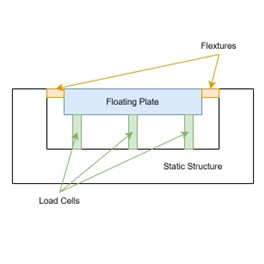
\includegraphics[width=0.4\linewidth]{static-structure-floating-plate-diagram.jpg}}
    \hspace{3em}
    \raisebox{-0.5\height}{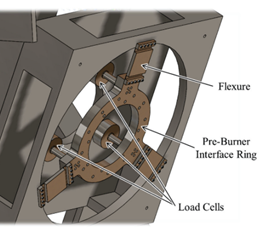
\includegraphics[width=0.4\linewidth]{static-structure-floating-plate-example.png}}
    \caption{\centering{A diagram of the static structure/floating plate configuration (left) and an example developed by Purdue's Zucrow Labs (right).}}
    \label{fig:static-floating-plate-example}
\end{figure}

\noindent\textit{Pros:}

The static structure/floating plate configuration is a very compact and straightforward design, stemming from the floating plate that transmits any thrust force directly to the load cells. This configuration reduces the number of moving parts in the system as a whole, which minimizes potential points of failure and makes the system easier to implement and maintain. This is particularly advantageous for facilities with limited space or those requiring a simple and straightforward solution.

One major strength of this configuration lies in its accuracy for axial force measurements while being able to minimize potential distortions caused by friction much easier. Compared to more complicated systems, this configuration reduces parasitic forces caused by structural deflections and alignment issues more efficiently as well. Because the test article is more closely anchored to the static structure, it is able to provide much more stability and ensure repeatable results over multiple tests.

With no sliding or other wear-prone components, this configuration would also be highly durable. This will ensure a much longer operational lifespan with minimal degradation or needed maintenance, which makes this configuration particularly suited for high-frequency testing environments. The lack of moving parts also makes the system less vulnerable to environmental factors, such as dust or debris, which could interfere with the operation of more complex configurations.

\noindent\textit{Cons:}

The first and foremost drawback of this configuration is how the floating plate will need to be specifically tailored to ensure it can integrate with each test article. While it is possible to keep integration methods the same between each test article, the floating plate design could limit the potential maximum size and thrust production that the test stand could handle. Retrofitting the test stand may require significant effort, making it less ideal for facilities conducting tests on a wide variety of test articles.

Another limitation lies in this configuration’s ability to handle dynamic or multi-axis forces. While a sliding rail configuration could be configured in a way to handle these extra forces, this design would only really be able to capture the axial force in a single direction without major modifications to the sensor system. In a project where budget is limited, compensating for the lack of dynamic force detection with multiple load cells may not be a great option.

There may also be a negative impact on this configuration caused by structural deformation and thermal effects. While the static structure provides a stable base for the test article, engines producing a particularly high thrust can induce minor deflections in the floating plate, potentially affecting the measurement accuracy. Addressing these issues often requires careful material selection and design, adding cost and complexity to what is otherwise a cost-effective and straightforward configuration.

\noindent\underline{Option 2: Sliding Rail Configuration}

A sliding rail configuration consists of a platform or carriage in which the test article is mounted on, and then this platform would slide along rails or bearings. The rails or bearings would be made out of low-friction materials (e.g. Teflon), to ensure accurate force transfer without any distortion caused by parasitic forces. The platform or carriage would then push into load cells attached to the rest of the test stand in order to measure the axial thrust generated by the test article. By putting the test article on rails or bearings, any forces produced would be constrained to the axial thrust direction, which allows the forces to be more accurately directed into the load cells.

\begin{figure}
    \centering
    \raisebox{-0.5\height}{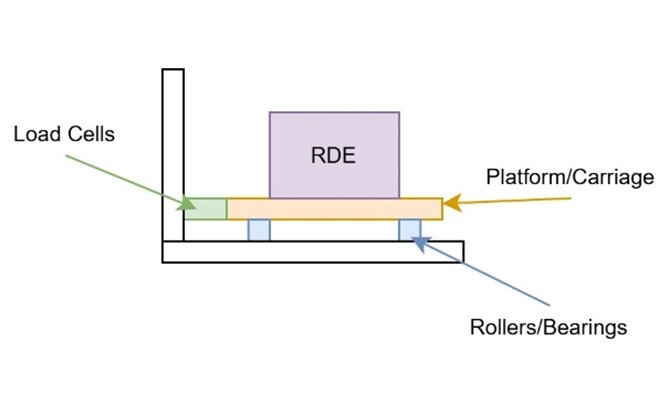
\includegraphics[width=0.4\linewidth]{sliding-rail-diagram.jpg}}
    \hspace{3em}
    \raisebox{-0.5\height}{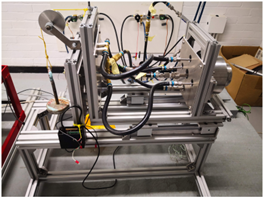
\includegraphics[width=0.4\linewidth]{sliding-rail-example.png}}
    \caption{\centering{A diagram of the sliding rail configuration (left) and an example developed by the University of Southampton (right).}}
    \label{fig:sliding-rail-example}
\end{figure}

\noindent\textit{Pros:}

The sliding rail configuration is one of the most ideal choices for isolating and accurately measuring axial forces generated by the test article. By constraining the test article’s motion to a single axis through rails or bearings, the system ensures that thrust is directed cleanly to the load cells, minimizing any interference from lateral forces. Using low-friction sliders or bearings also reduces the effect of parasitic forces such as friction. This allows for high-fidelity thrust measurements, where even minor distortions in force pathways could compromise the results.

This configuration also has the advantage of being modular and adaptable. The design can be easily adjusted to accommodate test articles of various sizes or thrust levels, which is particularly useful for a testing campaign with the goal of rapidly iterating over different designs, with each design able to be quickly integrated with the test stand numerous times. This dynamic testing environment of variable engine size/thrust can prove to be very useful for analyzing engine performance under realistic operating conditions.

The use of rails would also minimize structural distortion, as any thrust produced by the test article will be isolated to the rails and load cells, rather than being absorbed by a rigid frame. This will ensure consistent measurements, even for high-thrust engines, without the risk of inaccuracies from structural deformation. Additionally, the platform or sled in which the test article is integrated with will aid with thermal management by reducing heat transfer to the load cells and rest of the test stand structure.

\noindent\textit{Cons:}

One of the more major concerns that must be addressed with a sliding rail test stand configuration is the complexity of alignment. The rails and platform that the test article is on must be precisely aligned in order to ensure smooth motion and accurate force transmission into the load cells. Any improper alignment can introduce measurement errors, or worse, cause mechanical binding in the rail or bearing system. The demand for high precision increases initial installation time and the need for ongoing adjustments.

In addition, maintenance requirements could prove to increase the complexity required to implement the sliding rail solution. Any sliding components must be regularly inspected, cleaned, and lubricated in order to maintain their low-friction properties and ensure consistent performance. Over time, foreign object debris and wear and tear within the sliding components can lead to increased resistance, introducing additional parasitic forces that distort the thrust measurements.

While the nature of keeping the test article integrated to a separate platform will greatly reduce the amount of heat that transfers to the rest of the test stand, there could still be a non-negligible amount of heat that transfers to the rails. Any excessive heat that transfers to the sliding mechanism could potentially cause thermal expansion or warping, which would negatively affect the precise alignment and measurement accuracy. While this issue can be mitigated with proper material selection and thermal insulation techniques, it makes the sliding rail configuration less ideal for applications where simplicity and cost are major priorities.

% ----- CRITERIA & WEIGHTS -----
\begin{table}[H]
    \centering
    \singlespacing
    \small
    \caption{Load Transfer Configuration Trade Study - Evaluation Criteria}
    \label{tab:load_transfer_config_eval_criteria}

    \begin{subtable}[t]{\linewidth}
        \begin{tabularx}{\linewidth}{
            |>{\hsize=0.200\hsize}>{\centering\arraybackslash}X
            |>{\hsize=0.100\hsize}>{\centering\arraybackslash}X
            |>{\hsize=0.700\hsize}>{\centering\arraybackslash}X|
        }
            \hline
            \textbf{Decision Criteria} & \textbf{Weight} & \textbf{Reason} \\ \hline

            Complexity & 15\% & The design needs to be able to achieve its goals without unnecessary complexity in its assembly, serviceability, or maintenance, that can yield extra failure modes or unexpected behavior. \\ \hline
        
            Manufacturability & 15\% & The test stand should be able to be machined at the UCF machine shop without added difficulty. \\ \hline
        
            Risk & 20\% & While each option being considered has been tested in research previously, their specific adaptation to SABR can and will introduce unexpected risks, making the configuration choice paramount. \\ \hline
        
            Technical Performance & 50\% & The design’s ability to reliably handle and accurately measure the thrust produced by SABR are crucial for the success of the project. \\ \hline
        \end{tabularx}
        \smallskip
        \caption{Evaluation Criteria and Weights}
    \end{subtable}

\end{table}

\vspace{-2em}

% ----- COMPLEXITY SCALE -----
\begin{table}[H]
    \centering
    \singlespacing
    \small
    \ContinuedFloat

    \begin{subtable}[t]{\linewidth}
        \begin{tabularx}{\linewidth}{
            |>{\hsize=0.150\hsize}>{\centering\arraybackslash}X
            |>{\hsize=0.850\hsize}>{\centering\arraybackslash}X|
        }
            \hline
            \textbf{Score} & \textbf{Reason} \\ \hline
        
            4 & The design is simple in assembly, integration, use, and maintenance. \\ \hline
            
            3 & The design remains simple in assembly, integration and use, but maintenance requires some thought. \\ \hline
            
            2 & The design requires careful thought when integrating the engine or performing maintenance, but no critical issues arise from failure in these areas. \\ \hline
            
            1 & The design requires extreme care when assembling, integrating the engine, or performing maintenance, and poses a risk if these needs are not met. \\ \hline
        \end{tabularx}
        \smallskip
        \caption{Evaluation Scale - Complexity}
    \end{subtable}
\end{table}

\vspace{-2em}

% ----- MANUFACTURABILITY SCALE -----
\begin{table}[H]
    \centering
    \singlespacing
    \small
    \ContinuedFloat

    \begin{subtable}[t]{\linewidth}
        \begin{tabularx}{\linewidth}{
            |>{\hsize=0.150\hsize}>{\centering\arraybackslash}X
            |>{\hsize=0.850\hsize}>{\centering\arraybackslash}X|
        }
            \hline
            \textbf{Score} & \textbf{Reason} \\ \hline
        
            4 & The design remains functional with simple manufacturing methods and precise location of interacting components is not necessary. \\ \hline
            
            3 & The design remains functional with simple manufacturing methods and precise location and alignment is not necessary, but integration is critical to performance. \\ \hline
            
            2 & Manufacturing is complex but achievable within the means available; the design requires careful planning for integration and misalignment affects performance. \\ \hline
            
            1 & The design requires extreme care in integration and alignment of interacting components to maintain performance. Manufacturing is difficult and requires special tooling/machinery. \\ \hline
        \end{tabularx}
        \smallskip
        \caption{Evaluation Scale - Manufacturability}
    \end{subtable}
\end{table}

\vspace{-2em}

% ----- RISK SCALE -----
\begin{table}[H]
    \centering
    \singlespacing
    \small
    \ContinuedFloat

    \begin{subtable}[t]{\linewidth}
        \begin{tabularx}{\linewidth}{
            |>{\hsize=0.150\hsize}>{\centering\arraybackslash}X
            |>{\hsize=0.850\hsize}>{\centering\arraybackslash}X|
        }
            \hline
            \textbf{Score} & \textbf{Reason} \\ \hline
        
            4 & The design does not pose any risk to the structural stability of the test stand, and parasitic force distribution through the test stand is unlikely. \\ \hline
            
            3 & The design does not pose any risk to the structural stability of the test stand, but parasitic force distribution through the test stand is possible. \\ \hline
            
            2 & The design poses somewhat of a risk to the structural stability of the test stand, and parasitic force distribution is almost guaranteed. \\ \hline
            
            1 & The design poses an extreme risk to the structural stability of the test stand, and parasitic force distribution is almost guaranteed. \\ \hline
        \end{tabularx}
        \smallskip
        \caption{Evaluation Scale - Risk}
    \end{subtable}
\end{table}

\vspace{-2em}

% ----- TECHNICAL PERFORMANCE SCALE -----
\begin{table}[H]
    \centering
    \singlespacing
    \small
    \ContinuedFloat

    \begin{subtable}[t]{\linewidth}
        \begin{tabularx}{\linewidth}{
            |>{\hsize=0.150\hsize}>{\centering\arraybackslash}X
            |>{\hsize=0.850\hsize}>{\centering\arraybackslash}X|
        }
            \hline
            \textbf{Score} & \textbf{Reason} \\ \hline
        
            4 & The design exceeds the desired thrust measurement requirements for SABR performance. \\ \hline
            
            3 & The design meets the minimum thrust measurement requirements for SABR performance. \\ \hline
            
            2 & The design can meet the minimum thrust measurement requirements for SABR performance but requires a significant amount of post-processing on the load cell data. \\ \hline
            
            1 & The design is inefficient, ineffective, or otherwise fails to meet the desired thrust measurement requirements for SABR. \\ \hline
        \end{tabularx}
        \smallskip
        \caption{Evaluation Scale - Technical Performance}
    \end{subtable}
\end{table}

\vspace{-2em}

% ----- DECISION MATRIX (W/ COLORS) -----
% \begin{table}[H]
%     \centering
%     \singlespacing
%     \small
%     \begin{tabular}{|c|c|c|c|}

%         \hline
%         \multicolumn{2}{|c|}{\textbf{Criteria and Weights}}                         & \multicolumn{2}{|c|}{\textbf{Options and Scores}}                     \\ \hline

%         \textbf{Criteria}                                       & \textbf{Weights}  & \textbf{Static/Floating Plate}    & \textbf{Sliding Rail}             \\ \hline

%         \multicolumn{1}{|l|}{\textbf{Complexity}}               & 0.15              & \cellcolor{green!85!black} 4      & \cellcolor{green!15!yellow} 3     \\ \hline

%         \multicolumn{1}{|l|}{\textbf{Manufacturability}}        & 0.15              & \cellcolor{green!85!black} 4      & \cellcolor{green!15!yellow} 3     \\ \hline

%         \multicolumn{1}{|l|}{\textbf{Risk}}                     & 0.20              & \cellcolor{green!15!yellow} 3     & \cellcolor{green!85!black} 4      \\ \hline

%         \multicolumn{1}{|l|}{\textbf{Technical Performance}}    & 0.50              & \cellcolor{green!85!black} 4      & \cellcolor{green!85!black} 4      \\ \Xhline{2pt}

%         \multicolumn{1}{|l|}{\textbf{Weighted Scores}}          &                   & \cellcolor{green!85!black} 3.8    & \cellcolor{green!15!yellow} 3.7   \\ \hline

%     \end{tabular}
%     \caption{Load Transfer Configuration Study - Decision Matrix}
%     \label{tab:load_transfer_config_decision_matrix}
% \end{table}

% ----- DECISION MATRIX (W/O COLORS) -----
\begin{table}[H]
    \centering
    \singlespacing
    \small
    \begin{tabularx}{0.8\linewidth}{
        |>{\hsize=0.35\hsize}>{\centering\arraybackslash}X
        |>{\hsize=0.15\hsize}>{\centering\arraybackslash}X
        |>{\hsize=0.25\hsize}>{\centering\arraybackslash}X
        |>{\hsize=0.25\hsize}>{\centering\arraybackslash}X|
    }
        \hline
        \multicolumn{2}{|c|}{\textbf{Criteria and Weights}} & \multicolumn{2}{|c|}{\textbf{Options and Scores}} \\ \hline

        \textbf{Criteria} & \textbf{Weights} & \textbf{Hydraulic Calibration Structure} & \textbf{Mass-Pulley Calibration Structure} \\ \hline

        \multicolumn{1}{|l|}{\textbf{Complexity}} & 0.15 & 4 & 3 \\ \hline

        \multicolumn{1}{|l|}{\textbf{Manufacturability}} & 0.15 & 4 & 3 \\ \hline

        \multicolumn{1}{|l|}{\textbf{Risk}} & 0.20 & 3 & 4 \\ \hline

        \multicolumn{1}{|l|}{\textbf{Technical Performance}} & 0.50 & 4 & 4 \\ \Xhline{2pt}

        \multicolumn{1}{|l|}{\textbf{Weighted Scores}} & & 3.8 & 3.7 \\ \hline
        
    \end{tabularx}
    \caption{Load Transfer Configuration Study - Decision Matrix}
    \label{tab:load_transfer_config_decision_matrix}
\end{table}

\noindent\underline{Decision}

As shown by the decision matrix, the static structure/floating plate system is the optimal choice for the load transfer configuration. This system is much less complex from a design and integration standpoint, is much easier to manufacture and assemble, and is expected to yield the same results as the sliding rail configuration from a data measurement standpoint. Despite the slightly increased level of risk associated with this configuration, it is outweighed by its lack of complexity and cost. The decision to use a sliding rail configuration would yield similar results for thrust measurement, but the added complexity required to achieve that result is much less ideal.
\subsubsection{Load Cell Calibration Study}

In order to maintain accurate thrust measurement within a test stand built for rotating detonation engines, the functionality of the test stand’s load cells is critical. In an ideal test stand configuration, the entirety of the thrust produced by the test article on the stand would be transferred through the load cells, measuring the thrust to an extremely accurate degree. However, due to the nature of balancing efficient force distribution with structurally stable test stand designs, it is impossible to obtain an exact force reading using the load cells.

To solve this issue, the load cells can be calibrated prior to each test, to determine the difference between the amount of thrust determined by the load cells and the actual thrust produced by the test article. The calibration process is one of the most important aspects to consider of test stand design, as an improper load cell calibration would lead to inaccurate or completely non-sensical thrust readings. This trade study focuses on the nature of the test stand’s load cell calibration structure, and different potential configurations that will minimize any inaccuracies that could occur during the calibration process.

\noindent\underline{Option 1: Hydraulic Calibration Structure}

A hydraulic calibration structure utilizes a rigid framework designed to integrate directly with the test stand, or in some instances, directly with the test article itself in order to calibrate the load cells. At its core, the system features a high-pressure hydraulic ram capable of applying precise and repeatable loads onto the test stand or test article, mimicking the forces at specific locations that would be seen during a testing campaign. The structure’s rigidity minimizes deflection and ensures that the applied force can be accurately transmitted to the load cell under test and is designed to handle the high forces that can be associated with the testing of rotating detonation engines, ensuring calibration under conditions closely resembling actual operational scenarios.

\begin{figure}
    \centering
    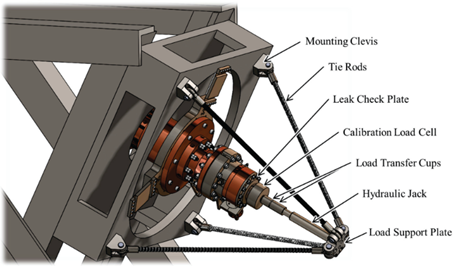
\includegraphics[width=0.6\linewidth]{hydraulic_calibration_example.png}
    \caption{An example of a hydraulic calibration structure developed by Purdue's Zucrow Labs.}
    \label{fig:hydraulic-calibration-example}
\end{figure}

\noindent\textit{Pros:}

If designed and assembled the right way, a hydraulic calibration structure would allow for exceptional accuracy and repeatability, which are critical for test stand applications. The hydraulic ram would be able to apply precise, controlled forces over a wide range, ensuring that the calibration data produced is highly reliable. With the incorporation of a rigid design, the deflection of the structure can be minimized, which helps to reduce measurement error as well. This precision makes the system suitable for higher-thrust applications where even minor inaccuracies could compromise data quality.

Another significant advantage of a hydraulic calibration structure is the system’s integration with the test stand and test article itself, ensuring that calibration occurs under realistic load conditions. By applying forces through the same paths and interfaces that will be used during actual tests, this method minimizes any structural differences that can occur between calibration and test configurations, such as misalignment or force path distortions. This approach results in a more accurate calibration, as it reflects the actual loading scenarios the load cells would experience during engine tests.

This structure also utilizes scalability and versatility to further enhance its utility. Hydraulic rams are capable of generating large amounts of force, which makes this design adaptable for calibrating a variety of load cells at different expected thrust amounts. Additionally, the ability to change the generated force of the hydraulic ram on the fly can allow precise calibration across the entire operational range of a load cell, ensuring accuracy across diverse test conditions. This flexibility can prove quite useful to testing campaigns looking to quickly iterate across different designs or setups.

\noindent\textit{Cons:}

One major drawback of the hydraulic calibration structure is its complexity and cost. The design and fabrication of a system capable of withstanding high forces without deflection demands significant resources. The hydraulic ram on its own could get quite expensive, in order to procure a ram that accurately provides the force required for an accurate load cell calibration. Additionally, the extra components required to mount the system to the test stand or test article can further add to the overall cost, as well as complexity required for the entire system to work.

Another limitation involves the significant setup and alignment time of the structure, which can lead to issues with operational delays. Ensuring proper alignment between the hydraulic ram, load cells, and calibration structure is crucial to avoid calibration errors, but this process can be fairly labor-intensive if designed poorly. Any issues that occur during setup can also introduce equipment errors or miscalibration of the hydraulic system itself, further adding to the overall calibration time.

This calibration structure also has the drawback of being unable to simulate dynamic or transient loads, which are critical for testing certain scenarios that could be experienced by the test article. While hydraulic systems excel at applying static forces, there is no efficient way to replicate any rapid thrust changes that could occur during a real-world testing campaign. This limitation could require the system to contain additional equipment in order to replicate these force conditions or ignore the calibration of dynamic thrust entirely.

\noindent\underline{Option 2: Mass-Pulley Calibration Structure}

A mass-pulley calibration structure involves attaching a mass pulley system to the test stand, with a procedure of applying known weights and measuring the resulting force read by the load cells. Specifically, a pulley would be placed on the back of the test stand, over which a string would be suspended below towards a platform in which the weights can be placed. Assuming the mass of the weights is exact, and the potential parasitic forces acting on the calibration system are known, the load cells in the test stand can be calibrated quite accurately.

\begin{figure}
    \centering
    \raisebox{-0.5\height}{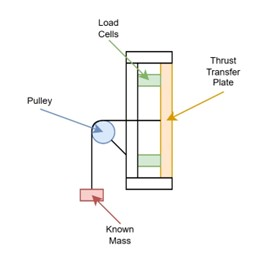
\includegraphics[width=0.4\linewidth]{mass-pulley-calibration-diagram.jpg}}
    \hspace{3em}
    \raisebox{-0.5\height}{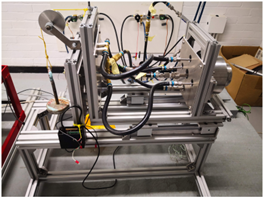
\includegraphics[width=0.4\linewidth]{mass-pulley-calibration-example.png}}
    \caption{\centering{A diagram of the pulley-and-weight calibration structure (left) and an example developed by the University of Southampton (right).}}
    \label{fig:mass-pulley-calibration-example}
\end{figure}

\noindent\textit{Pros:}

The use of a mass-pulley system for calibration is a lot more straightforward and cost-effective than most other solutions. It primarily relies on readily available components like calibrated weights, pulleys, and cables, making it easy to assemble and replicate. Any other required components would likely be able to be fabricated with ease as well. This simplicity reduces the potential for complex mechanical or electronic failures during the calibration process and ensures that the setup can be quickly adapted for different ranges of applied forces.

The mass-pulley calibration system is also much more well-suited for low-force ranges compared to high-force ranges. The accuracy with these lower forces means that the calibration system will be able to much more reliably measure thrust data closer to the range in which a standard small-scale rotating detonation engine will operate. Producing data in this critical range will allow the engine performance the be evaluated much more confidently.

Additionally, this calibration system’s modular design allows for much easier adjustments to the range of forces in which the load cells need to be calibrated to. Changing the force being applied to the load cell during the calibration process is as easy as adding to or changing the known weight being suspended below the pulley. This flexibility makes the structure suitable for a variety of thrust measurement scenarios, whether quickly calibrating between different iterations of a test article or between different expected thrusts that could be produced.

\noindent\textit{Cons:}

The use of a mass-pulley system for calibration is a lot more straightforward and cost-effective than most other solutions. It primarily relies on readily available components like calibrated weights, pulleys, and cables, making it easy to assemble and replicate. Any other required components would likely be able to be fabricated with ease as well. This simplicity reduces the potential for complex mechanical or electronic failures during the calibration process and ensures that the setup can be quickly adapted for different ranges of applied forces.

The mass-pulley calibration system is also much more well-suited for low-force ranges compared to high-force ranges. The accuracy with these lower forces means that the calibration system will be able to much more reliably measure thrust data closer to the range in which a standard small-scale rotating detonation engine will operate. Producing data in this critical range will allow the engine performance the be evaluated much more confidently.

Additionally, this calibration system’s modular design allows for much easier adjustments to the range of forces in which the load cells need to be calibrated to. Changing the force being applied to the load cell during the calibration process is as easy as adding to or changing the known weight being suspended below the pulley. This flexibility makes the structure suitable for a variety of thrust measurement scenarios, whether quickly calibrating between different iterations of a test article or between different expected thrusts that could be produced.

% ----- CRITERIA & WEIGHTS -----
\begin{table}[H]
    \centering
    \singlespacing
    \small
    \caption{Load Cell Calibration Trade Study - Evaluation Criteria}
    \label{tab:load_cell_calibration_eval_criteria}

    \begin{subtable}[t]{\linewidth}
        \begin{tabularx}{\linewidth}{
            |>{\hsize=0.200\hsize}>{\centering\arraybackslash}X
            |>{\hsize=0.100\hsize}>{\centering\arraybackslash}X
            |>{\hsize=0.700\hsize}>{\centering\arraybackslash}X|
        }
            \hline
            \textbf{Decision Criteria} & \textbf{Weight} & \textbf{Reason} \\ \hline

            Complexity & 15\% & The design needs to be able to achieve its goals without unnecessary complexity in its assembly, serviceability, or maintenance, that can yield extra failure modes or unexpected behavior. \\ \hline
        
            Manufacturability & 15\% & The test stand should be able to be machined at the UCF machine shop without added difficulty. \\ \hline
        
            Risk & 20\% & While each option being considered has been tested in research previously, their specific adaptation to SABR can and will introduce unexpected risks, making the configuration choice paramount. \\ \hline
        
            Technical Performance & 50\% & The design’s ability to reliably handle and accurately measure the thrust produced by SABR are crucial for the success of the project. \\ \hline
        \end{tabularx}
        \smallskip
        \caption{Evaluation Criteria and Weights}
    \end{subtable}

\end{table}

\vspace{-2em}

% ----- COMPLEXITY SCALE -----
\begin{table}[H]
    \centering
    \singlespacing
    \small
    \ContinuedFloat

    \begin{subtable}[t]{\linewidth}
        \begin{tabularx}{\linewidth}{
            |>{\hsize=0.150\hsize}>{\centering\arraybackslash}X
            |>{\hsize=0.850\hsize}>{\centering\arraybackslash}X|
        }
            \hline
            \textbf{Score} & \textbf{Reason} \\ \hline
        
            4 & Calibration involves minimal setup and few components, requiring basic tools or fixtures. \\ \hline
            
            3 & Calibration requires specialized equipment but remains relatively straightforward, the procedure involves multiple steps but is not resource intensive. \\ \hline
            
            2 & Calibration involves more advanced systems, requiring precise alignment and controlled environments. \\ \hline
            
            1 & Calibration uses dynamic or highly specialized systems and requires significant expertise. \\ \hline
        \end{tabularx}
        \smallskip
        \caption{Evaluation Scale - Complexity}
    \end{subtable}
\end{table}

\vspace{-2em}

% ----- MANUFACTURABILITY SCALE -----
\begin{table}[H]
    \centering
    \singlespacing
    \small
    \ContinuedFloat

    \begin{subtable}[t]{\linewidth}
        \begin{tabularx}{\linewidth}{
            |>{\hsize=0.150\hsize}>{\centering\arraybackslash}X
            |>{\hsize=0.850\hsize}>{\centering\arraybackslash}X|
        }
            \hline
            \textbf{Score} & \textbf{Reason} \\ \hline
        
            4 & The design uses standard components that require minimal customization, and any fabrication involves basic machining with minimal cost and lead times. \\ \hline
            
            3 & The design requires some custom components requiring some intermediate level machining but are not highly specialized or difficult to produce. \\ \hline
            
            2 & The design relies on custom-engineered parts or systems and requires more advanced techniques to fabricate. \\ \hline
            
            1 & The design incorporates highly specialized materials and would require extensive prototyping and specialized facilities. \\ \hline
        \end{tabularx}
        \smallskip
        \caption{Evaluation Scale - Manufacturability}
    \end{subtable}
\end{table}

\vspace{-2em}

% ----- RISK SCALE -----
\begin{table}[H]
    \centering
    \singlespacing
    \small
    \ContinuedFloat

    \begin{subtable}[t]{\linewidth}
        \begin{tabularx}{\linewidth}{
            |>{\hsize=0.150\hsize}>{\centering\arraybackslash}X
            |>{\hsize=0.850\hsize}>{\centering\arraybackslash}X|
        }
            \hline
            \textbf{Score} & \textbf{Reason} \\ \hline
        
            4 & The calibration process involves few safety or operational risks, and features simple, fail-safe mechanisms. \\ \hline
            
            3 & The calibration process involves some operational risks, but they are manageable with standard precautions. Safety concerns can be easily mitigated through training. \\ \hline
            
            2 & The calibration process involves significant operational risks, and safety hazards requiring strict protocols and regular maintenance exist. \\ \hline
            
            1 & The calibration process involves highly complex components with catastrophic failure modes. System failure could lead to severe safety incidents or irreparable damage. \\ \hline
        \end{tabularx}
        \smallskip
        \caption{Evaluation Scale - Risk}
    \end{subtable}
\end{table}

\vspace{-2em}

% ----- TECHNICAL PERFORMANCE SCALE -----
\begin{table}[H]
    \centering
    \singlespacing
    \small
    \ContinuedFloat

    \begin{subtable}[t]{\linewidth}
        \begin{tabularx}{\linewidth}{
            |>{\hsize=0.150\hsize}>{\centering\arraybackslash}X
            |>{\hsize=0.850\hsize}>{\centering\arraybackslash}X|
        }
            \hline
            \textbf{Score} & \textbf{Reason} \\ \hline
        
            4 & The design exceeds the desired thrust measurement requirements for SABR performance. \\ \hline
            
            3 & The design meets the minimum thrust measurement requirements for SABR performance. \\ \hline
            
            2 & The design can meet the minimum thrust measurement requirements for SABR performance but requires a significant amount of post-processing on the load cell data. \\ \hline
            
            1 & The design is inefficient, ineffective, or otherwise fails to meet the desired thrust measurement requirements for SABR. \\ \hline
        \end{tabularx}
        \smallskip
        \caption{Evaluation Scale - Technical Performance}
    \end{subtable}
\end{table}

\vspace{-2em}

% ----- DECISION MATRIX -----
\begin{table}[H]
    \centering
    \singlespacing
    \small
    \begin{tabularx}{0.8\linewidth}{
        |>{\hsize=0.35\hsize}>{\centering\arraybackslash}X
        |>{\hsize=0.15\hsize}>{\centering\arraybackslash}X
        |>{\hsize=0.25\hsize}>{\centering\arraybackslash}X
        |>{\hsize=0.25\hsize}>{\centering\arraybackslash}X|
    }
        \hline
        \multicolumn{2}{|c|}{\textbf{Criteria and Weights}} & \multicolumn{2}{|c|}{\textbf{Options and Scores}} \\ \hline

        \textbf{Criteria} & \textbf{Weights} & \textbf{Hydraulic Calibration Structure} & \textbf{Mass-Pulley Calibration Structure} \\ \hline

        \multicolumn{1}{|l|}{\textbf{Complexity}} & 0.25 & 3 & 4 \\ \hline

        \multicolumn{1}{|l|}{\textbf{Manufacturability}} & 0.15 & 2 & 4 \\ \hline

        \multicolumn{1}{|l|}{\textbf{Risk}} & 0.10 & 3 & 4 \\ \hline

        \multicolumn{1}{|l|}{\textbf{Technical Performance}} & 0.50 & 4 & 3 \\ \Xhline{2pt}

        \multicolumn{2}{|l|}{\textbf{Weighted Scores}} & \textbf{3.35} & \textbf{3.50} \\ \hline
        
    \end{tabularx}
    \caption{Load Cell Calibration Trade Study - Decision Matrix}
    \label{tab:load_cell_calibration_decision_matrix}
\end{table}

\noindent\underline{Decision}

As shown by the decision matrix, a mass-pulley system is the ideal choice for the test stand calibration structure. It is less complex in its design, much easier to manufacture, and slightly less risky than the option of a hydraulic calibration structure, but slightly less accurate in its ability to calibrate to a high enough accuracy. Despite the lower accuracy, the mass-pulley system is still more than capable of meeting the minimum project requirements, and its shortcomings are easily outweighed by its lack of complexity and cost. On the other hand, the use of the hydraulic calibration structure would likely yield load cell calibration to a higher accuracy, but with the drawbacks of a much more complex and risky system.

\subsection{Fluid System and Controls Trade Studies}

\newpage
\begin{flushleft}
    \singlespacing
    \bibliographystyle{IEEEtran}
    \bibliography{refs}
\end{flushleft}

\end{document}